%-----------------------------------------------------------------------
% Cgins : Incompressible Navier Stokes Solver
% 
%           User Guide
%
%-----------------------------------------------------------------------
\documentclass{article}
% \usepackage[bookmarks=true]{hyperref} 
\usepackage[bookmarks=true,colorlinks=true,linkcolor=blue]{hyperref}

% \input documentationPageSize.tex
\hbadness=10000 
\sloppy \hfuzz=30pt

% \voffset=-.25truein
% \hoffset=-1.25truein
% \setlength{\textwidth}{7in}      % page width
% \setlength{\textheight}{9.5in}    % page height

\usepackage{calc}
\usepackage[margin=1.in]{geometry}

%% \input homeHenshaw

\usepackage{amsmath}
\usepackage{amssymb}

\usepackage{verbatim}
\usepackage{moreverb}

\usepackage{graphics}    
\usepackage{epsfig}    
\usepackage{calc}
\usepackage{ifthen}
\usepackage{float}
% the next one cause the table of contents to disappear!
% * \usepackage{fancybox}

%\input{pstricks}\input{pst-node}
%\input{colours}

% define the clipFig commands:
% \input clipFig.tex
\usepackage{tikz}
\input ../common/trimFig.tex

\newcommand{\bogus}[1]{}  % begin a section that will not be printed

\usepackage{makeidx} % index
\makeindex
\newcommand{\Index}[1]{#1\index{#1}}


% ---- we have lemmas and theorems in this paper ----
\newtheorem{assumption}{Assumption}
\newtheorem{definition}{Definition}

% \newcommand{\ovFigures}{\homeHenshaw/OvertureFigures}
% \newcommand{\docFigures}{\homeHenshaw/OvertureFigures}
% \newcommand{\figures}{\homeHenshaw/res/OverBlown/docFigures}
% \newcommand{\obFigures}{\homeHenshaw/res/OverBlown/docFigures}  % note: local version for OverBlown

\newcommand{\Overture}{{\bf Overture\ }}
% \newcommand{\insDocDir}{\homeHenshaw/overtureFramework/cgDoc/ins}
\newcommand{\insDocDir}{.}

% -------------  -------------------
\newcommand{\Solver}{Cgins}
\newcommand{\solver}{cgins}

\newcommand{\bfss}{\sffamily\bfseries}


% *** See http://www.eng.cam.ac.uk/help/tpl/textprocessing/squeeze.html
% By default, LaTeX doesn't like to fill more than 0.7 of a text page with tables and graphics, nor does it like too many figures per page. This behaviour can be changed by placing lines like the following before \begin{document}

\renewcommand\floatpagefraction{.9}
\renewcommand\topfraction{.9}
\renewcommand\bottomfraction{.9}
\renewcommand\textfraction{.1}   
\setcounter{totalnumber}{50}
\setcounter{topnumber}{50}
\setcounter{bottomnumber}{50}


% ***************************************************************************
\begin{document}


% -----definitions-----
\input ../common/wdhDefinitions.tex

\def\ud     {{    U}}
\def\pd     {{    P}}

\newcommand{\mbar}{\bar{m}}
\newcommand{\Rbar}{\bar{R}}
\newcommand{\Ru}{R_u}         % universal gas constant
\newcommand{\Div}{\grad\cdot}
\newcommand{\tauv}{\boldsymbol{\tau}}
\newcommand{\sumi}{\sum_{i=1}^n}
\newcommand{\dt}{{\Delta t}}

\vglue 5\baselineskip
\begin{flushleft}
{\Large
{\bf Cgins} User Guide: An Overture Solver for the Incompressible Navier--Stokes Equations on Composite Overlapping Grids, \\
}
\vspace{2\baselineskip}
William D. Henshaw,\\
Department of Mathematical Sciences, \\
Rensselaer Polytechnic Institute, \\
Troy, NY, USA, 12180.
% \footnote{This work was performed under the auspices of the U.S. Department of Energy (DOE) by
% Lawrence Livermore National Laboratory under Contract DE-AC52-07NA27344 and by 
% DOE contracts from the ASCR Applied Math Program.}  \\
% Centre for Applied Scientific Computing  \\
% Lawrence Livermore National Laboratory      \\
% Livermore, CA, 94551.  \\
% henshaw@llnl.gov \\
% http://www.llnl.gov/casc/people/henshaw \\
% http://www.llnl.gov/casc/Overture\\
\vspace{\baselineskip}
\today\\
% \vspace{\baselineskip}
% LLNL-SM-455851

\vspace{4\baselineskip}

\noindent{\bf Abstract:}
This is the user guide for Cgins.  Cgins is a program that can be used to solve
incompressible fluid flow problems in complex geometry in two and three
dimensions using composite overlapping grids. It is built upon the \Overture
object-oriented framework.  Cgins solves the incompressible Navier-Stokes
equations using a pressure-Poisson formulation. Second-order accurate and
fourth-order accurate approximations are available.  Cgins can be used to
\begin{itemize}
  \item solve problems in two and three dimensional complex domains,
  \item solve problems on moving grids (specified motion and rigid body motion), 
  \item solve temperature dependent flows with buoyancy using the Boussinesq approximation,  
  \item solve axisymmetric flows.
%   \item solve for visco-plastic flows (Bingham plastics). 
\end{itemize} 
This user guide describes how to get started and how to run Cgins. Various examples are given.
The options for running the code along with specification of initial conditions and
boundary conditions are described.

\end{flushleft}

\clearpage
\tableofcontents
% \listoffigures

\clearpage
\section{Introduction}

Cgins\footnote{Thanks to Kyle Chand for all his contributions to Cgins including
the development of the AFS algorithm.} is an incompressible fluid flow solver for overlapping grids built upon
the \Overture framework~\cite{Brown97},\cite{Henshaw96a},\cite{iscope97}.
More information about
{\bf Overture} can be found on the \Overture home page, {\tt http://www.llnl.gov/\-casc/\-Overture}.


Cgins
solves the incompressible Navier-Stokes
equations using a pressure-Poisson formulation~\cite{ICNS}. Second-order accurate and
fourth-order accurate approximations are available.  Cgins can be used to
\begin{itemize}
  \item solve problems in two and three dimensional complex domains,
  \item solve problems on moving grids (specified motion and rigid body motion), 
  \item solve temperature dependent flows with buoyancy using the Boussinesq approximation,  
  \item solve axisymmetric flows.
%   \item solve for visco-plastic flows (Bingham plastics). 
\end{itemize} 
This user guide describes how to get started and how to run Cgins. Various examples are given.
The options for running the code along with specification of initial conditions and
boundary conditions are described.

\vskip\baselineskip
The Cgins solver is found in the {\tt ins} directory in the {\bf cg} distribution and has
sub-directories
\begin{description}
 \item[{\tt bin}] : contains the executable, cgins. You may want to put this directory in your path.
 \item[{\tt check}] : contains regression tests.
 \item[{\tt cmd}] : sample command files for running cgins, see section (\ref{sec:demo}).
%  \item[{\tt doc}] : dcoumentation.
 \item[{\tt lib}] : contains the Cgins library, {\tt libCgins.so}.
 \item[{\tt src}] : source files 
\end{description}


\noindent
Other documents of interest that are available through the \Overture home page are
\begin{itemize}
\item The Cgins Reference Manual~\cite{CginsReferenceManual} for detailed descriptions of the
      equations, algorithms and discretizations.
\item The overlapping grid generator, {\tt Ogen}, \cite{OGEN}. Use this program to make grids for cgins.
\item Mapping class documentation : {\ff mapping.tex}, \cite{MAPPINGS}. Many of the mappings that
   are used to create an overlapping grid are documented here. 
\item Interactive plotting : {\ff PlotStuff.tex}, \cite{PLOTSTUFF}.
\item {\tt Oges} overlapping grid equation solver, used by Cgins to solve implicit time stepping
    equations and the Poisson equation for the pressure, \cite{OGES}.
\end{itemize}

% \vskip.5\baselineskip
% \noindent{\bf Acknowledgements:} Thanks to Kyle Chand for all his contributions to Cgins including
%    his development of the AFS algorithm. 

% -------------------------------------------------------------------------------------------------------
\subsection{Basic steps}\index{basic steps}
Here are the basic steps to solve a problem with Cgins.
\begin{enumerate}
  \item Generate an overlapping grid with ogen. Make the grid with 2 ghost lines (this is the default).
  \item Run cgins (note lowercase 'c', found in the {\tt bin/cgins} directory) 
        and choose the PDE you want to solve.
  \item Assign the boundary conditions and initial conditions.
  \item Choose the parameters for the PDE (Reynold's number, Mach number etc.)
  \item Choose run time parameters, time to integrate to, time stepping method etc.
  \item Compute the solution (optionally plotting the results as the code runs).
  \item When the code is finished you can look at the results (provided you saved a
     `show file') using {\tt plotStuff}.
\end{enumerate}
The commands that you enter to run cgins can be saved in a \Index{command file} (by default
they are saved in the file `cgins.cmd'). This command file can be used to re-run
the same problem by typing `cgins file.cmd'. The command file can be edited to change parameters.

To get started you can run one of the demo's that come with cgins, these are 
explained next in section~(\ref{sec:demo}).

Papers that describe some of the \Index{algorithms} used in Cgins include
\begin{enumerate}
  \item {\sl A Fourth-Order Accurate Method for the Incompressible
            {N}avier-{S}tokes Equations on Overlapping Grids} \cite{ICNS},
  \item {\em A Split-Step Scheme for the Incompressible {Navier-Stokes} Equations}~\cite{splitStep2003},
  \item {\sl Composite Overlapping Meshes for the Solution of Partial Differential Equations}
        \cite{CGNS},
  \item {\sl Analysis of a Difference Approximation for the Incompressible
            Navier-Stokes Equations} \cite{INSDIV}.
         
\end{enumerate}

  
\begin{figure}[hbt]
\begin{center}
%  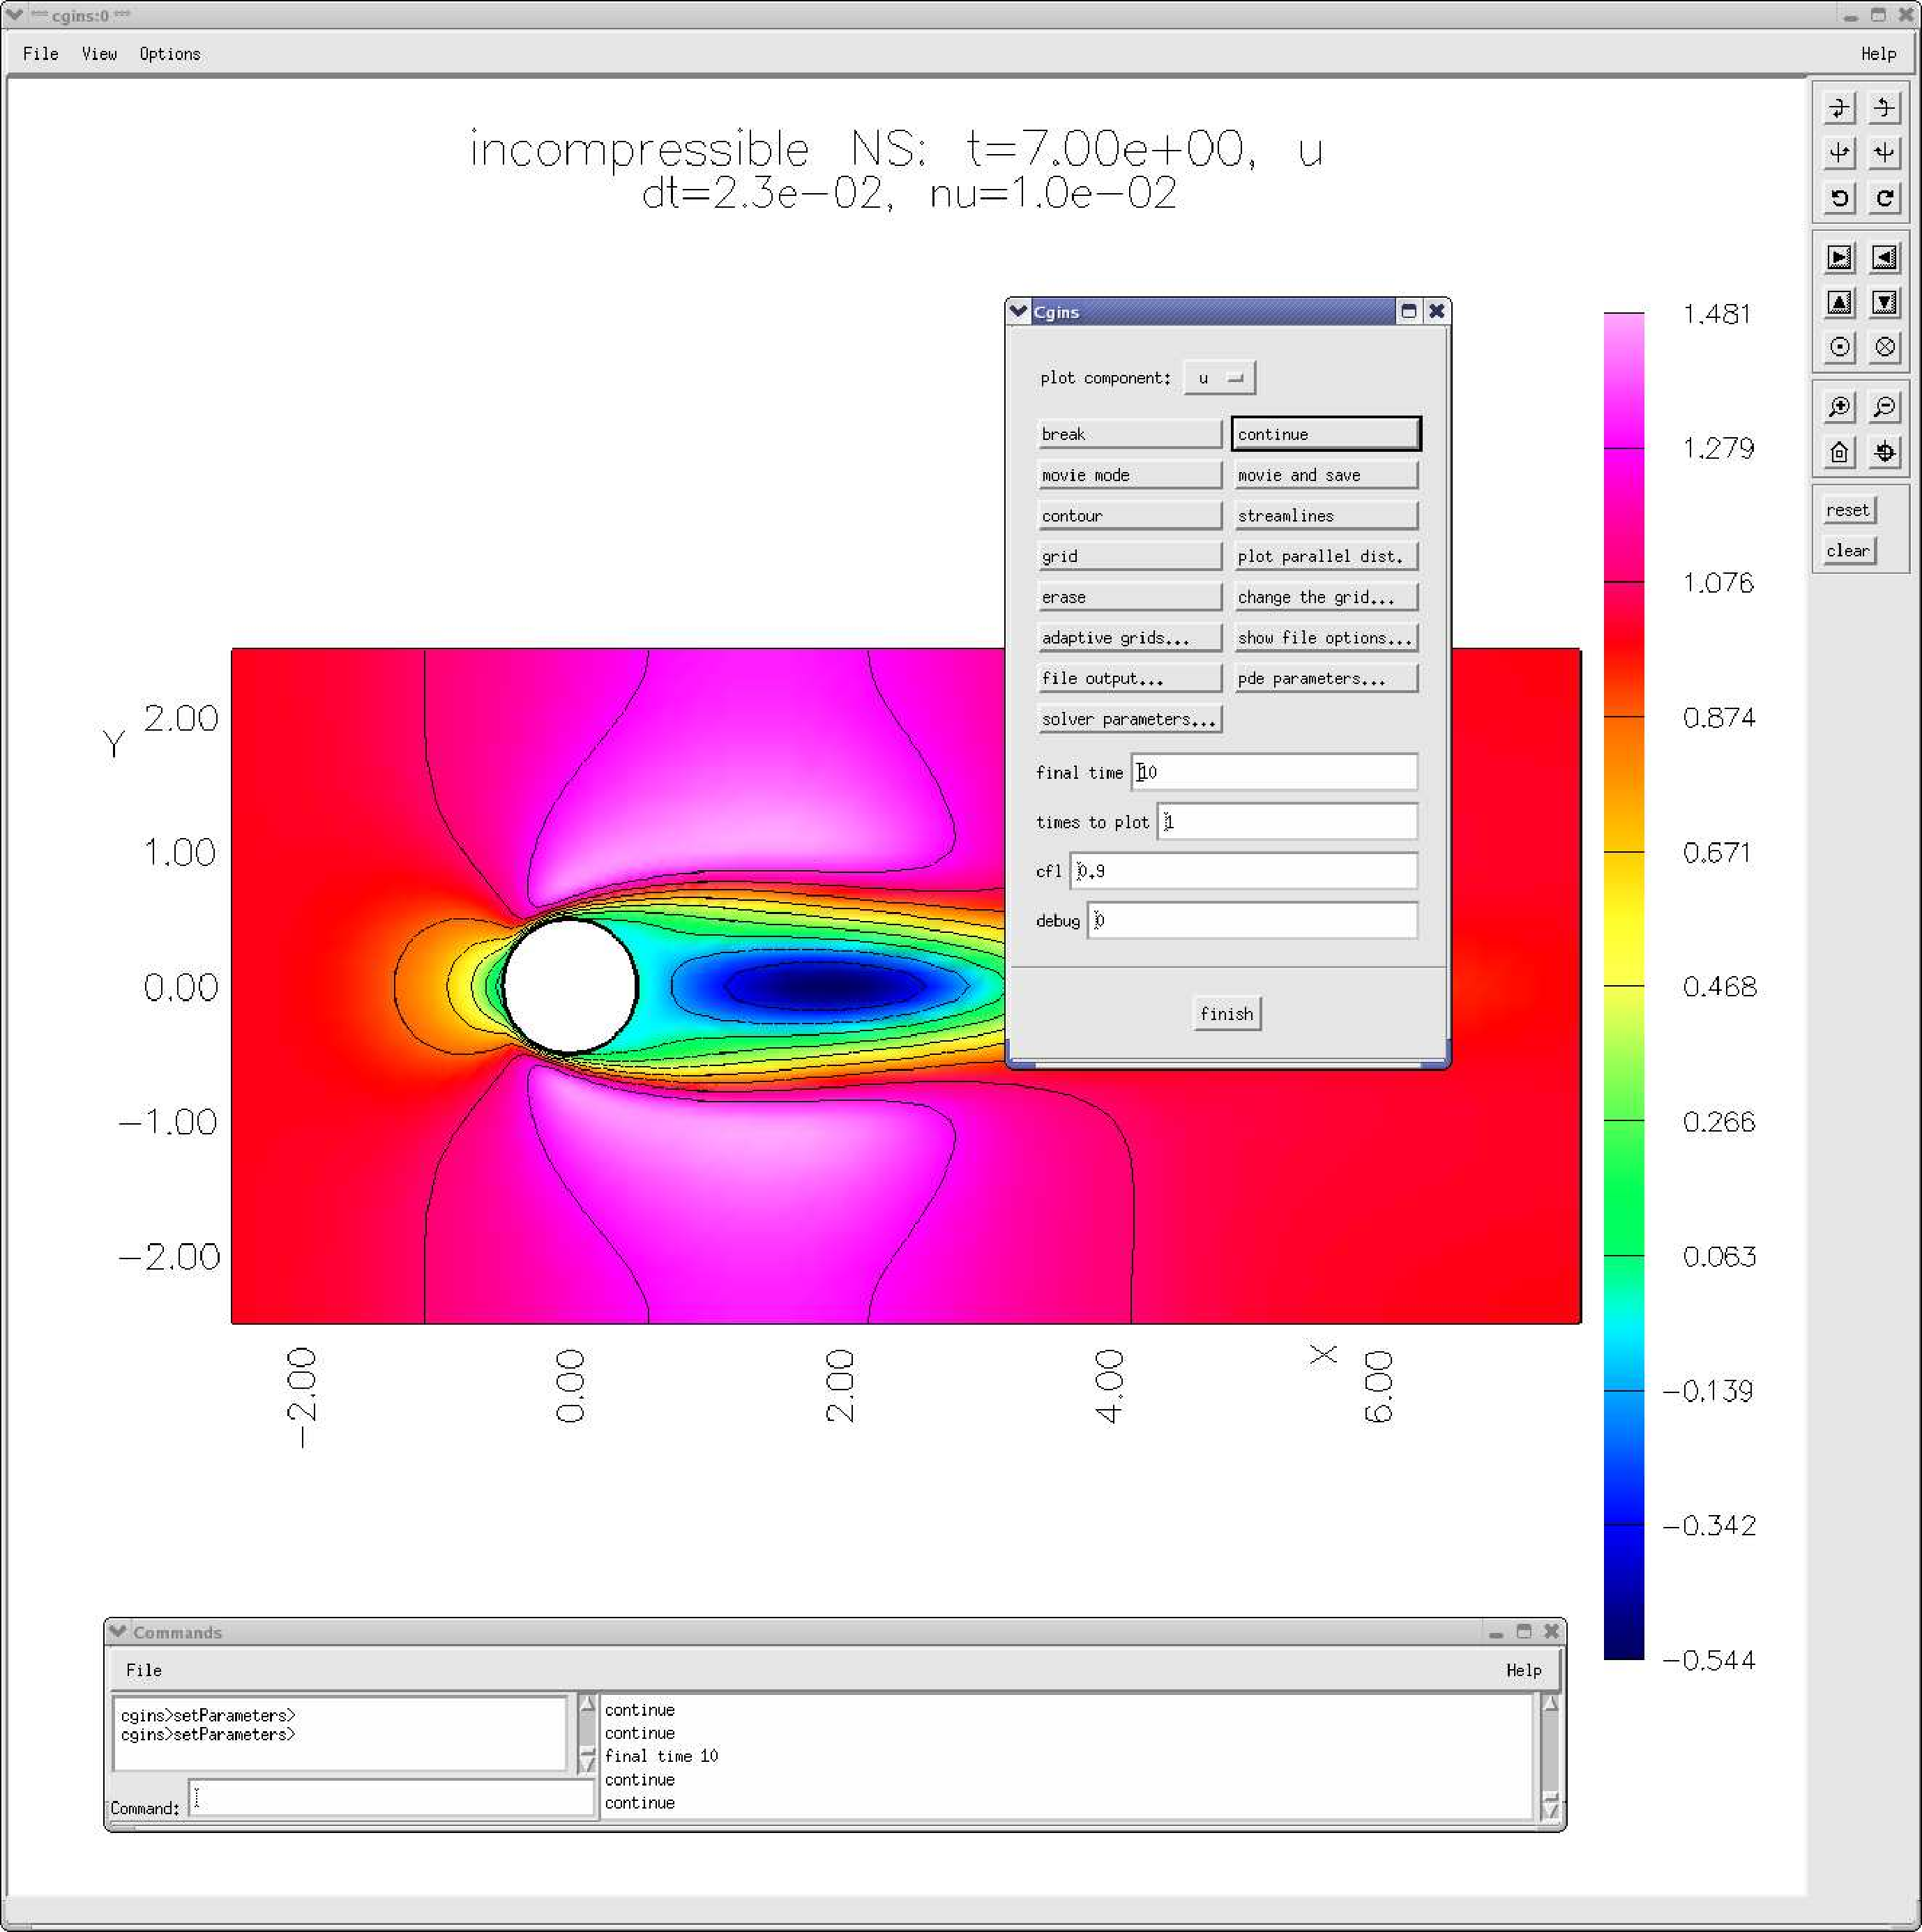
\epsfig{file=cginsScreen.eps,width=.95\linewidth}  \\
  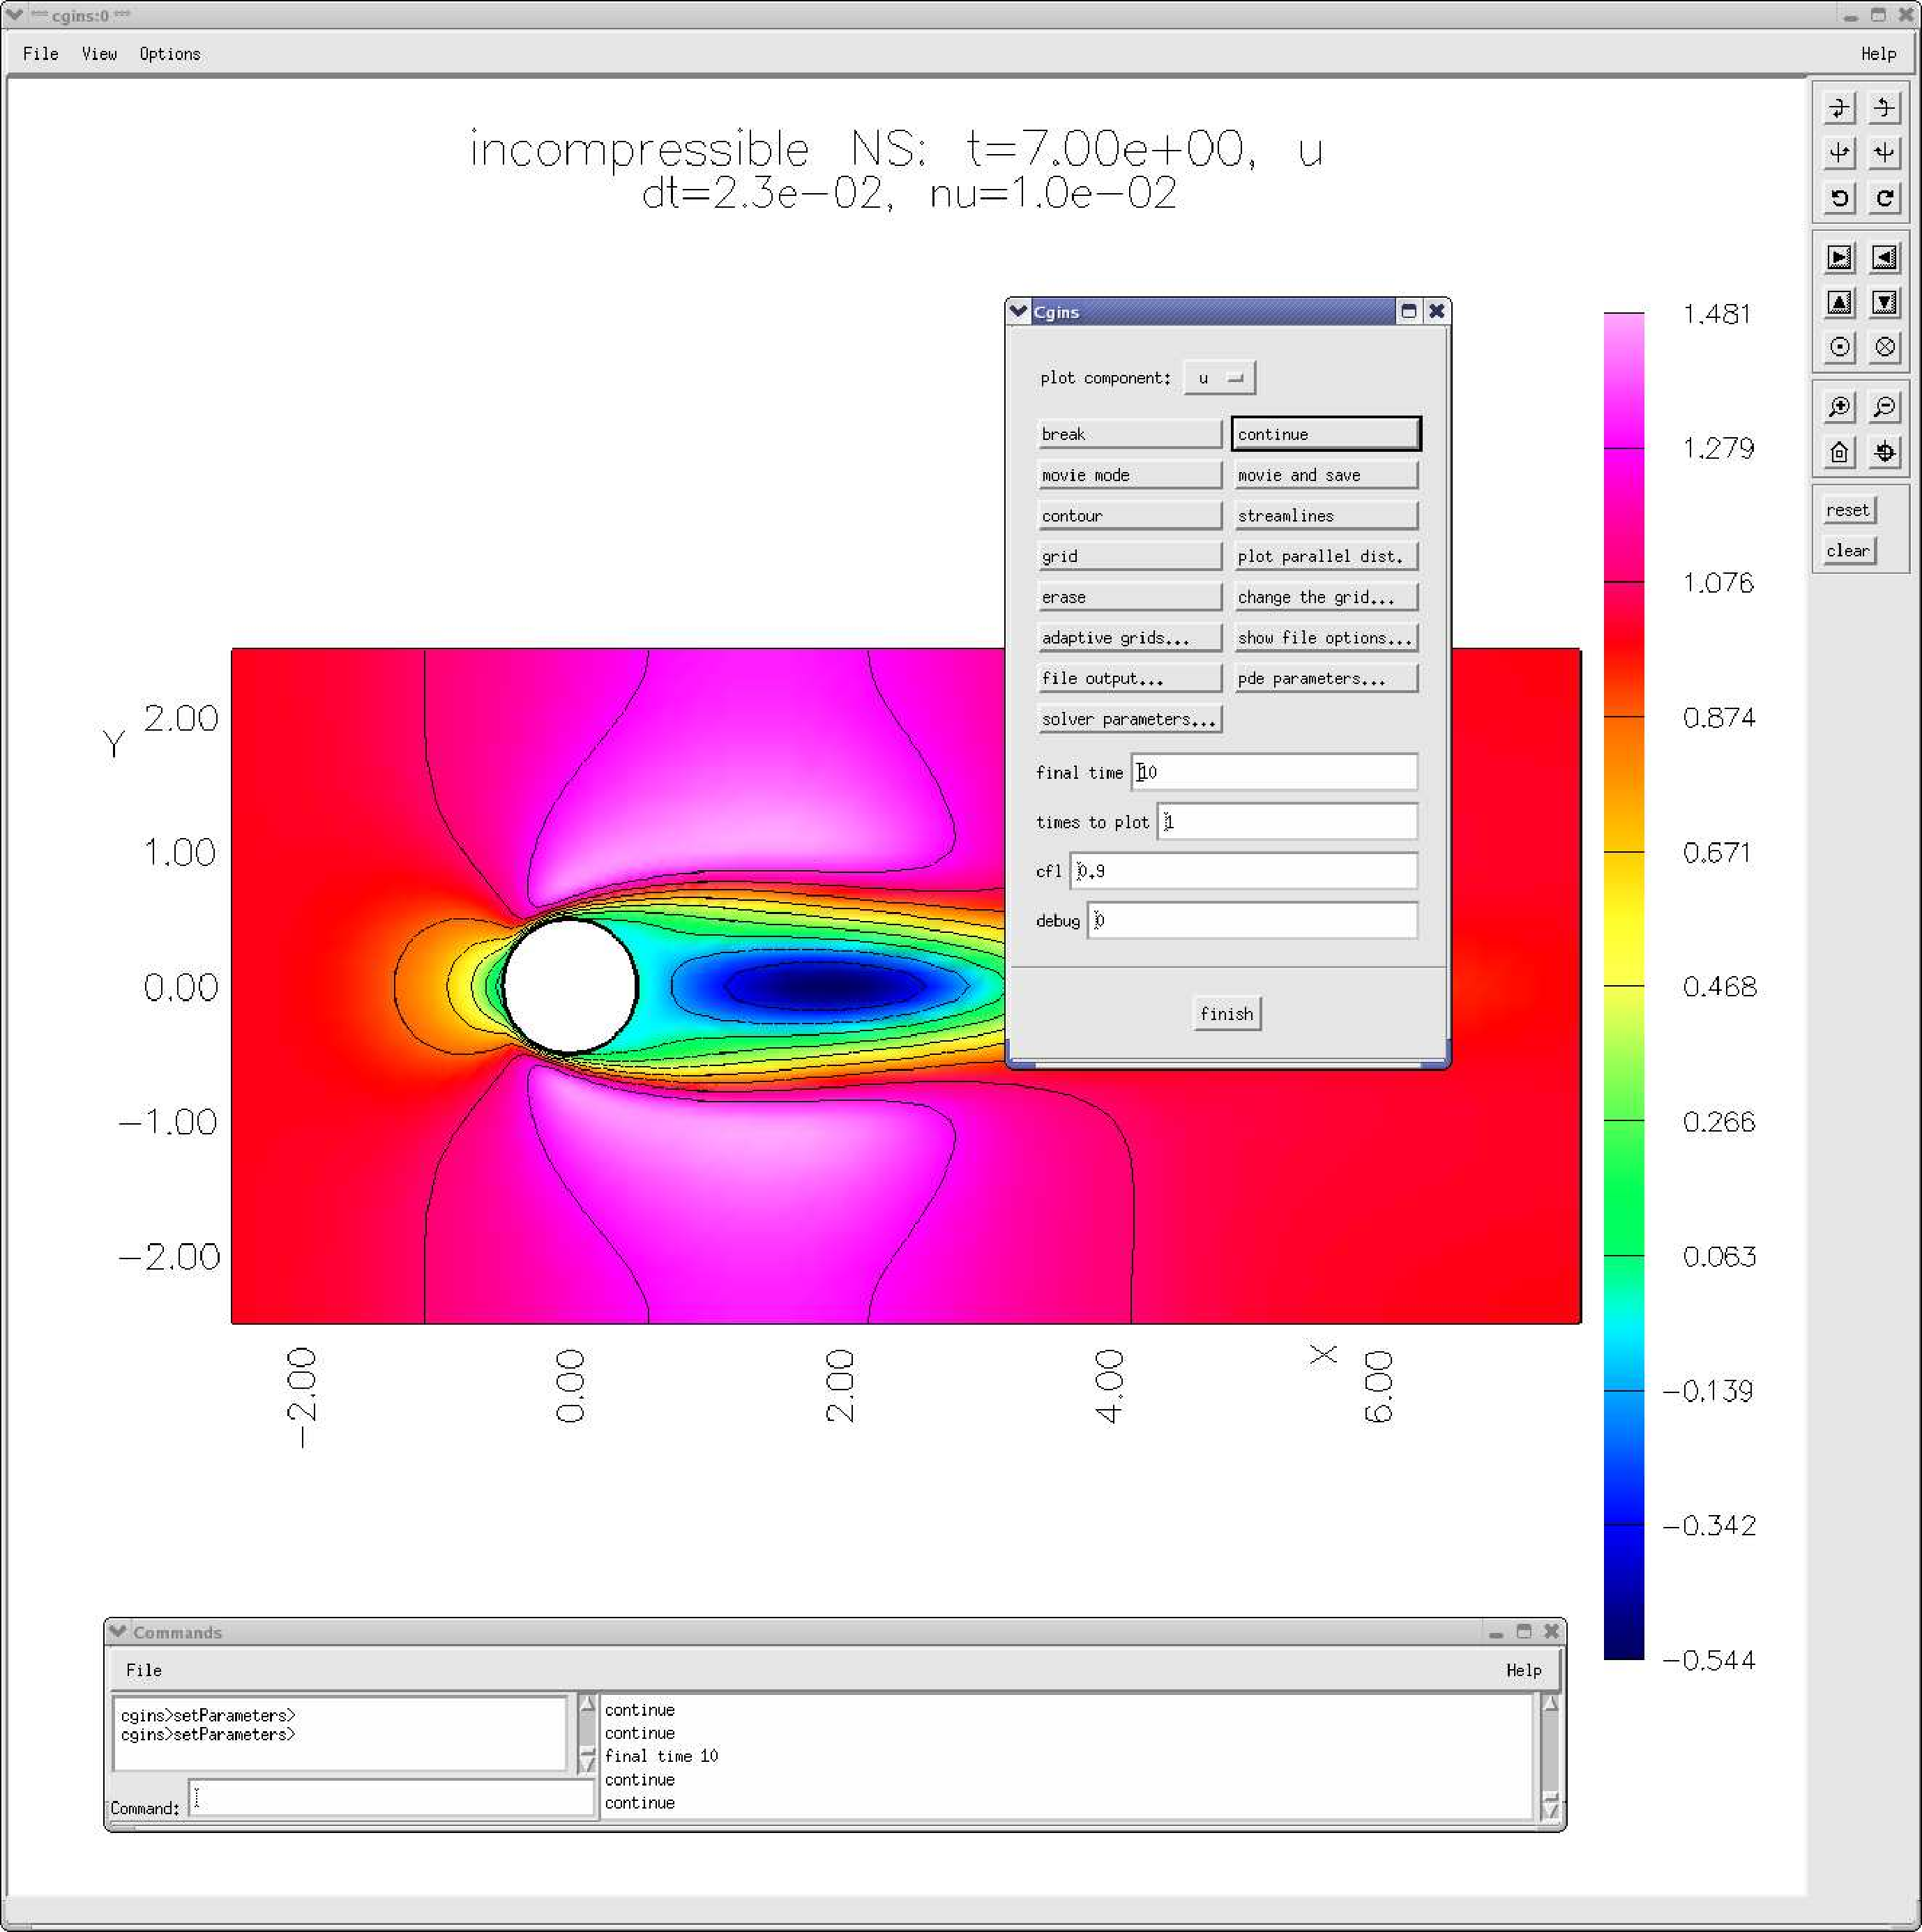
\includegraphics[width=.75\linewidth]{cginsScreen} \\
  \caption{Snapshot of cgins showing the run time dialog menu. }
  \end{center} 
  \label{fig:runTimeScreen}
\end{figure}

\clearpage
% ------------------------------------------------------------------------------------------------
\section{Sample command files for running cgins} \label{sec:demo}

Command files are supported throughout the Overture. They are files
that contain lists of commands. These commands can initially be saved
when the user is interactively choosing options.  The \Index{command files}
can then be used to re-run the job. Command files can be edited and
changed.

In this section we present a number of command files that can be used
to run cgins. See the file {\tt cg/ins/cmd/Readme} for a list and brief description of
the command files found in {\tt cg/ins/cmd}. 

% ------------------------------------------------------------------------------------------------
\subsection{Running a command file}

Given a \Index{command file} for cgins such as {\tt cylinder.cmd}, found in {\tt
cmd/cylinder.cmd}, one can type `{\tt cgins cylinder.cmd}' to run this command
file . You can also just type `{\tt cgins cylinder}, leaving off the {\tt
.cmd} suffix. Typing `{\tt cgins noplot cylinder}' will run without
interactive graphics (unless the command file turns on graphics). Note that here
it is assumed that the {\tt bin} directory is in your path so that the {\tt
cgins} command is found when you type it's name. The Cgins sample
command files will automatically look for an overlapping grid in the {\tt
Overture/sampleGrids} directory, unless the grid is first found in the location
specified in the command file.

When you run a command file a graphics screen will appear and after some
processing the run-time dialog should appear and the initial conditions will be
plotted, see Figure~\ref{fig:runTimeScreen}. The program will also print out some information about the problem
being solved. 
Many of the command files such as the stirring-stick problem, {\tt stir.cmd},
can take command line arguments.  For example, here
are two command lines that run a problem with different grids and parameters:
\begin{verbatim}
  cgins stir -g=stir.hdf -nu=.05 -tf=1. -tp=.025 
  cgins stir -g=stir2.hdf -nu=.01 -tf=1. -tp=.002 -rate=8.
\end{verbatim}
See the comments at the top of {\tt stir.cmd} for further explanation and examples.

% ------------------------------------------------------------------------------------------------
\subsection{Incompressible flow past a cylinder in a long channel}

The command file {\tt cg/ins/cmd/cylinder.cmd} can be used
to compute the incompressible flow past a cylinder in a channel, see Figure~\ref{fig:cylinder}.
This example uses the grid {\tt Overture/\-sampleGrids/cilc.hdf}.

{
\begin{figure}[hbt]
\newcommand{\figWidtha}{7.5cm}
\newcommand{\trimfiga}[2]{\trimPlotb{#1}{#2}{.0}{.0}{.1}{.0}}
\begin{center}
\begin{tikzpicture}[scale=1]
  \useasboundingbox (0,.75) rectangle (15.,7);  % set the bounding box (so we have less surrounding white space)
  \draw ( 0.0,0.0) node[anchor=south west,xshift=-4pt,yshift=+0pt] {\trimfiga{./fig/ob_ins_cylinder_sl0}{\figWidtha}};
  \draw ( 7.7,0.0) node[anchor=south west,xshift=-4pt,yshift=+0pt] {\trimfiga{./fig/ob_ins_cylinder_sl50}{\figWidtha}};
  % 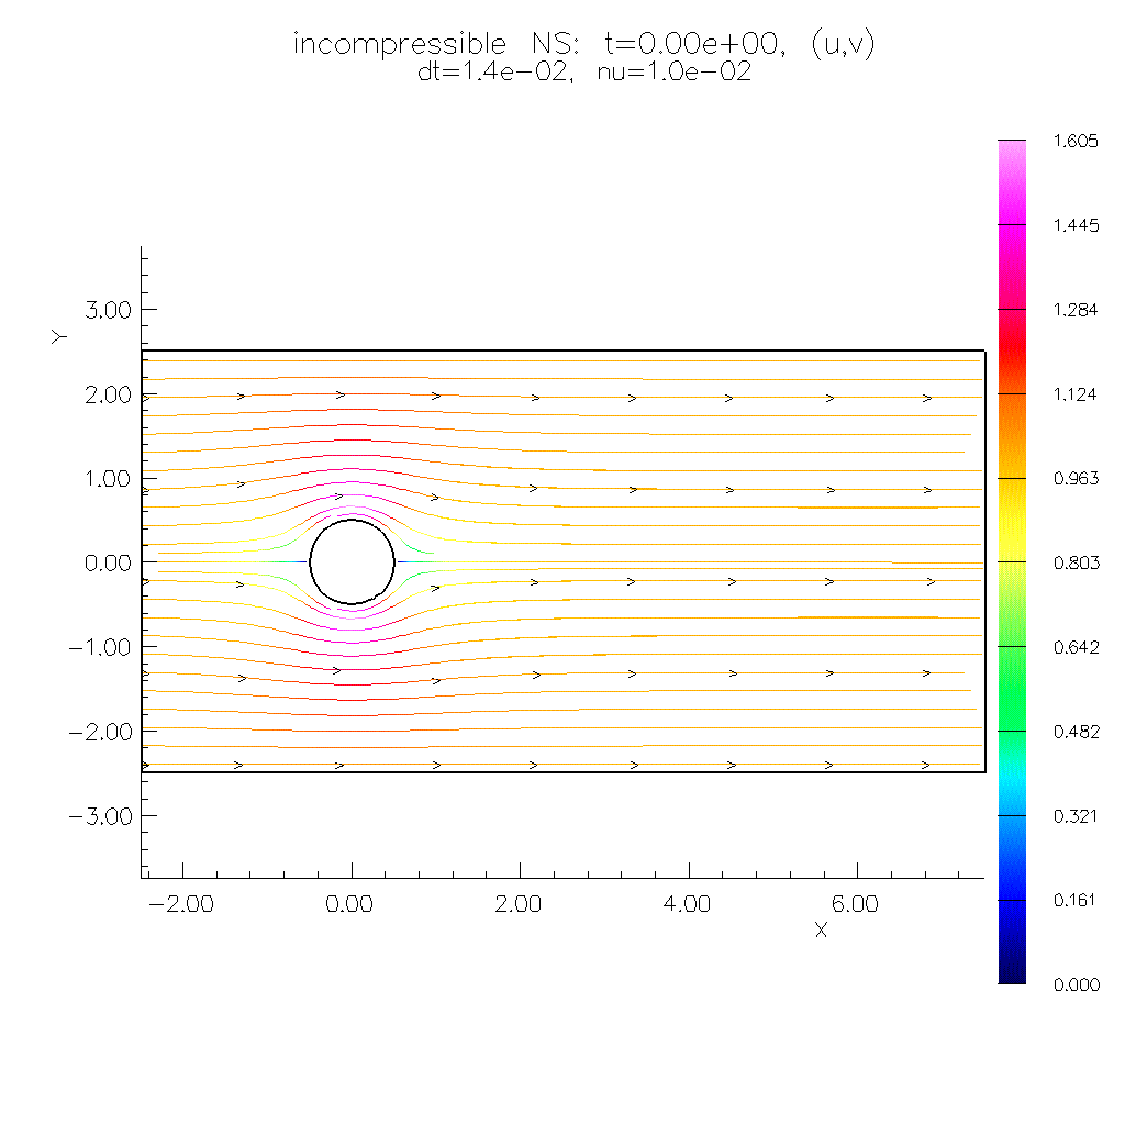
\includegraphics[width=.475\linewidth]{./fig/ob_ins_cylinder_sl0}
  % 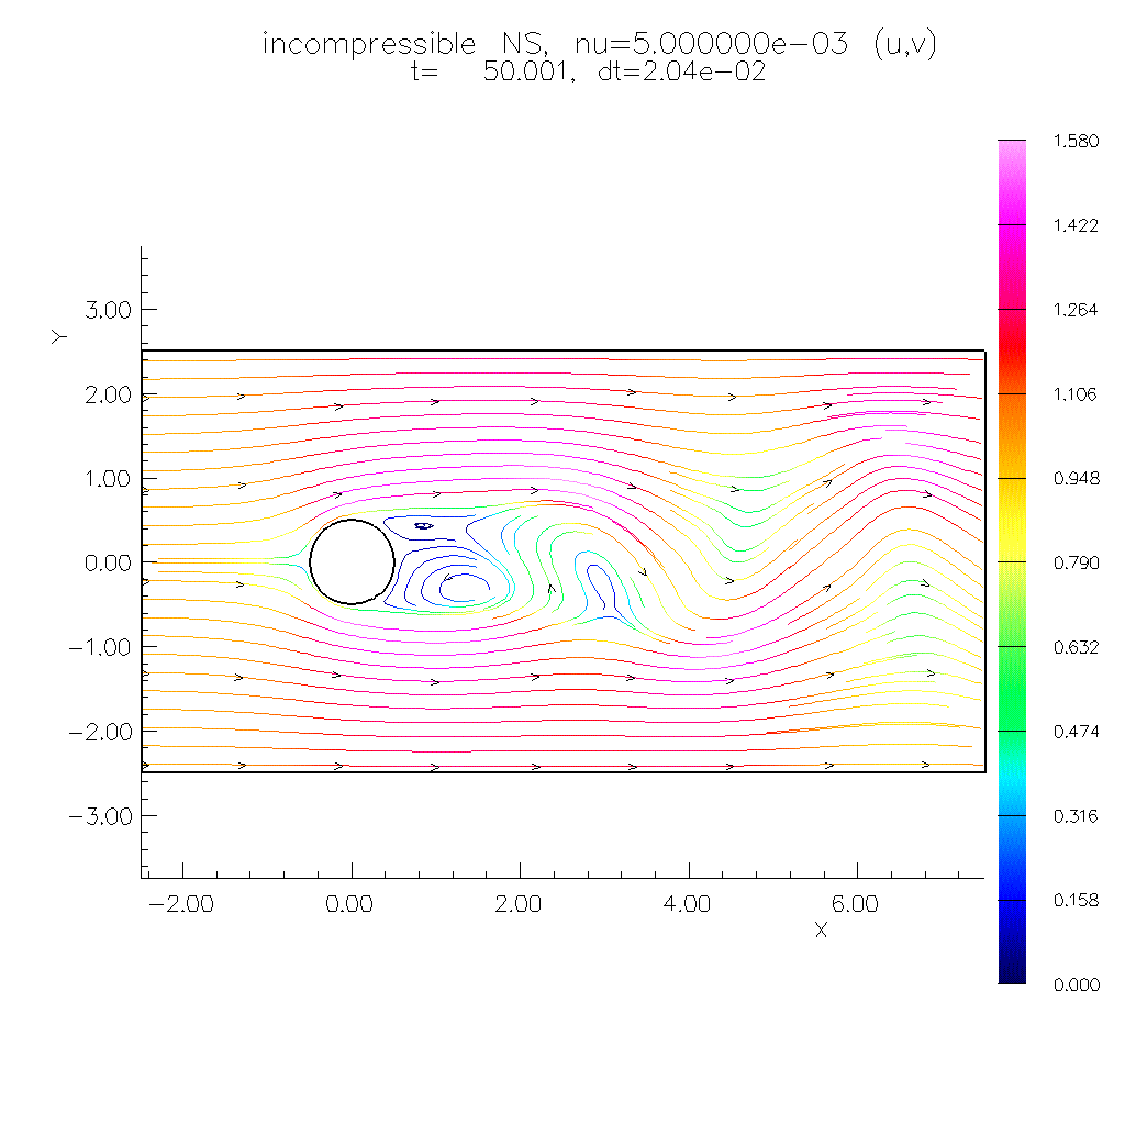
\includegraphics[width=.475\linewidth]{./fig/ob_ins_cylinder_sl50}
% grid:
%\draw[step=1cm,gray] (0,0) grid (15,7.);
\end{tikzpicture}
\end{center} 
\caption{Incompressible flow around a cylinder. Left: the initial conditions are obtained by
    projecting a uniform flow, $(u,v)=(1,0)$. Right: the solution at time $t=40$.}
  \label{fig:cylinder}
\end{figure}
}

To run cgins with the {\tt cylinder.cmd} script, type
\begin{flushleft}
  \tt cgins \$ins/cmd/cylinder.cmd
\end{flushleft}
% At this point choose {\tt continue} or {\tt movie mode}.
Then choose one of:
\begin{flushleft}
  {\tt continue} : to advance to the next output time. \\
  {\tt plot component} : to plot different solution components. \\
  {\tt streamlines} : to plot streamlines (choose {\tt erase first}). \\
  {\tt grid} : to plot the grid (choose {\tt erase first}). \\
  {\tt movie mode} : to run and plot. \\
  {\tt break} : to break from movie mode. \\
  {\tt final time 50.} : to increase the final time.
\end{flushleft}
Further description of the options available in the
run time dialog can be found in Section~\ref{sec:runTimeDialog}.
\vskip.5\baselineskip
{\bf Note:} If cgins cannot find the cilc.hdf grid file, you can generate it with: 
\begin{flushleft}
  \tt ogen -noplot \$sampleGrids/cilc.cmd
\end{flushleft}

Here are some more examples using the command line arguments to choose different options:
\begin{flushleft}
  {\tt cgins cylinder -g=cilc.hdf -tf=50. -tp=1.} : specify the grid, final time and time to plot. \\
  {\tt cgins cylinder -g=cilce2.order4 -tf=50. -tp=.1 -nu=.01} : solve a fourth-order accurate 
         problem~\footnote{By default, Cgins determines the order of accuracy from the grid: the order of accuracy
         of the grid is specified when the grid is constructed using ogen. A fourth-order accurate grid will have two
     layers of interpolation points (to support a 5 point stencil) and use high-order accurate interpolation with a
     interpolation stencil width of 5 in each direction.}. 
\end{flushleft}


% To run this command file from the {\tt cmd} directory type {\tt `cgins cylinder'}
% (or {\tt ../bin/cgins cylinder'} if you have not set your path). 

\noindent {\bf Notes:}
\begin{itemize}
  \item If the overlapping grid file, {\tt cilc.hdf} is not found then you may need to specify
        the full path to its location, {\tt -g=/home/henshaw/myGrids/cilc.hdf}. The suffix {\tt `.hdf'}
        is optional when specifying grids as Overture will tack on {\tt `.hdf'} if necessary.
        If Cgins does not  find the file specified it will also by default look for the file in the
        {\tt Overture/\-sampleGrids} directory. 
  \item The initial conditions are assigned to be a uniform flow, $(u,v)=(1,0)$. 
        These initial conditions are projected to nearly satisfy $\grad\cdot\uv=0$
        by using the {\tt `project initial conditions'} option (see~\cite{CginsReferenceManual}).
  \item The time-stepping method is chosen so that the grid around the cylinder
         uses implicit time-stepping while the back-ground grid uses explicit time-stepping.
        This was done for efficiency. The grids around the cylinder have small grid spacings so that
        implicit time stepping is especially useful. The back-ground grid does not have small grid spacings
        so there is not much of an advantage in using implicit time stepping.
        By treating the back-ground grid explicitly the implicit time stepping equations 
        require less storage and cpu time to solve.
  \item By default the implicit equations and elliptic pressure equation are solved with a direct sparse solver. This usually
        is the best approach for 2D problems, unless the grids get large, since the matrix is factored
        only once. In later examples it will be shown how to specify an iterative method.
\end{itemize}


% ------------------------------------------------------------------------------------------------
\clearpage
\subsection{Flow past two cylinders using different time-stepping methods}

In this section we compute the flow past two cylinders in order
to demonstrate the use of some different time-stepping methods for Cgins.
These time-stepping methods include the explicit predictor-corrector (PC), the implicit predictor-corrector (IM)
the approximate factored scheme (AFS), and the (pseudo) steady-state line solver (SS). 
Figure~\ref{fig:tcilc} shows two grids at different resolutions(-factor=2,4 with -order=2 as described below) and the solution (on a grid -factor=8, -order=4). 
{
\begin{figure}[hbt]
\newcommand{\figWidtha}{8.cm}
\newcommand{\trimfiga}[2]{\trimPlotb{#1}{#2}{.02}{.02}{.275}{.275}}
\begin{center}
\begin{tikzpicture}[scale=1]
  \useasboundingbox (0,.75) rectangle (16.5,7.75);  % set the bounding box (so we have less surrounding white space)
  \draw ( 0.0,3.75) node[anchor=south west,xshift=-4pt,yshift=+0pt] {\trimfiga{./fig/tcilc2Grid}{\figWidtha}};
  \draw ( 0.0,0.0 ) node[anchor=south west,xshift=-4pt,yshift=+0pt] {\trimfiga{./fig/tcilc4Grid}{\figWidtha}};
% 
  \draw ( 8.25,3.75) node[anchor=south west,xshift=-4pt,yshift=+0pt] {\trimfiga{./fig/tcilc4_vor_t10p0}{\figWidtha}};
  \draw ( 8.25,0.0 ) node[anchor=south west,xshift=-4pt,yshift=+0pt] {\trimfiga{./fig/tcilc4_SL_t10p0}{\figWidtha}};
  % 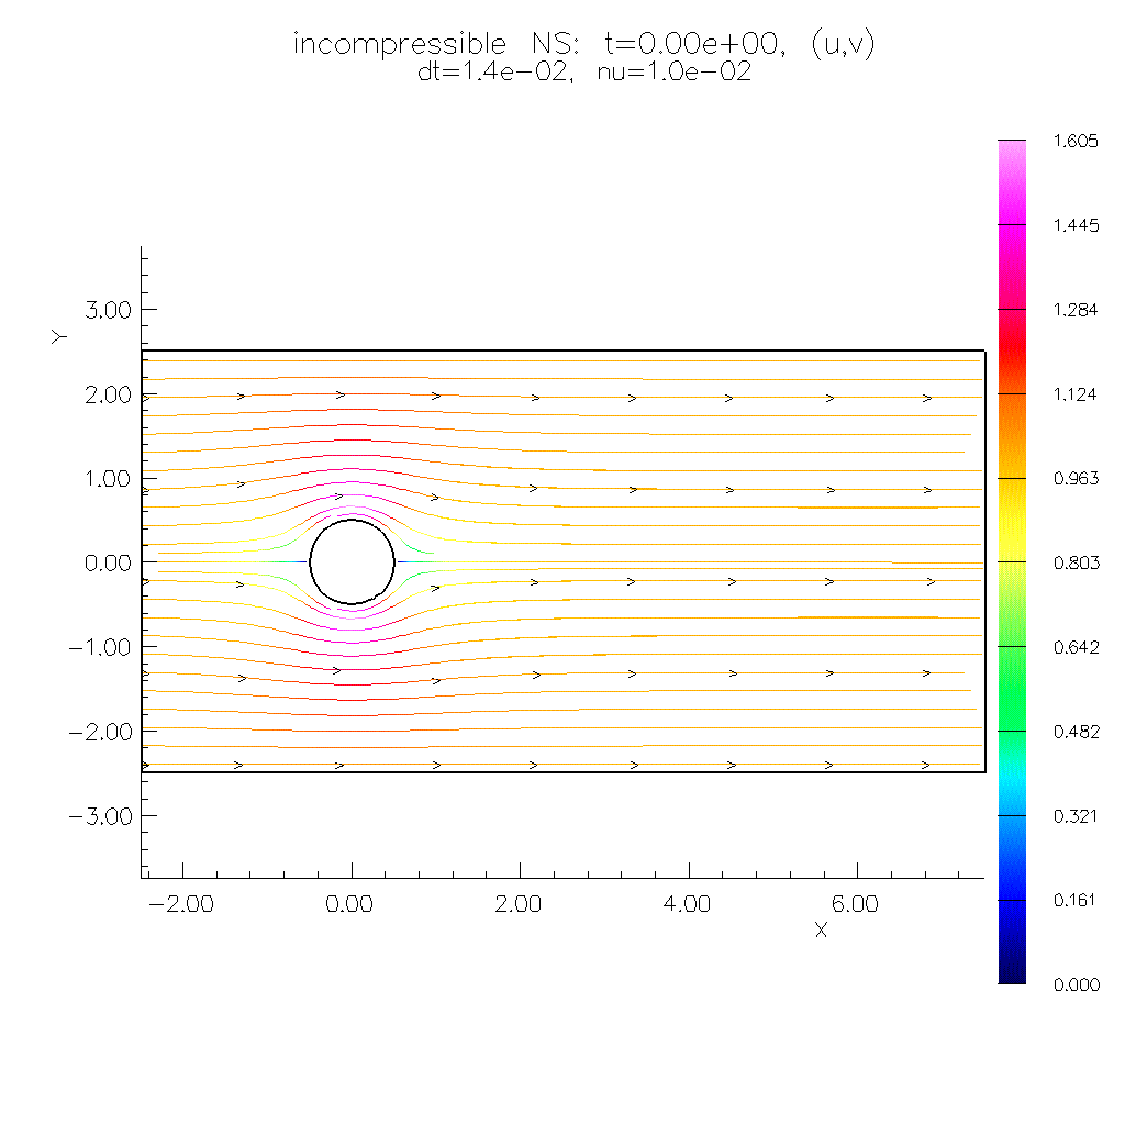
\includegraphics[width=.475\linewidth]{./fig/ob_ins_cylinder_sl0}
  % 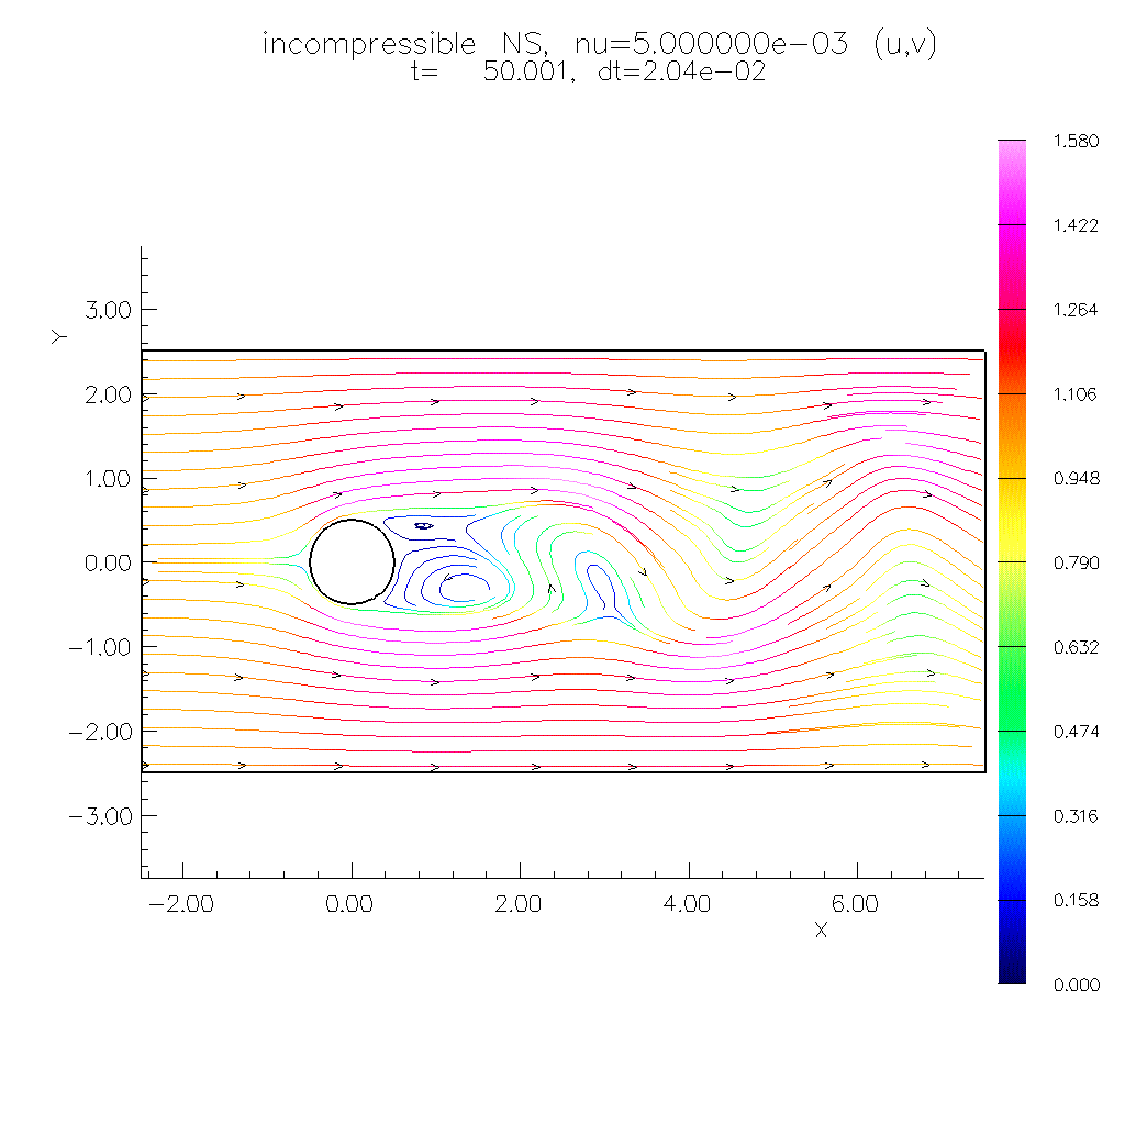
\includegraphics[width=.475\linewidth]{./fig/ob_ins_cylinder_sl50}
% grid:
% \draw[step=1cm,gray] (0,0) grid (16.5,8.);
\end{tikzpicture}
\end{center} 
\caption{Incompressible flow past two cylinders. Left: overlapping grids at two resolutions.
         Right: vorticity and streamlines at time $t=10$, (AFS24, tcilce8.order4.ml3, $\nu=10^{-4}$).}
  \label{fig:tcilc}
\end{figure}
}

The examples in this section use the Cgins command file {\tt cg/ins/cmd/tcilc.cmd}.
This script optionally takes numerous command line arguments that can be used to change parameters: 
\begin{flushleft}\tt
 cgins [-noplot] tcilc -g=<grid-name> -nu=<> -tf=<> -tp=<> -show=<> -debug=<> -project=[0|1] -ad2=[0|1] -ad4=[0|1] -ad41=<> -ad42=<> ... 
         -ts=[pc|im|afs|ss] -solver=[best|mg|yale] -psolver=[best|mg|yale] -rtolp=<>  \\
~~ \\
\quad -tf, -tp: final time and times to plot. \\
\quad -show : name of show file. \\
\quad -project : 1=project initial conditions to be approximate divergence free. \\
\quad -ad2 : 1=turn on 2nd-order artificial dissipation. \\
\quad -ad4 : 1=turn on 4th-order artificial dissipation. \\
\quad -ad41, -ad42 : coefficients in fourth-order non-linear dissipation. \\
\quad -ts : time-stepping method. \\
\quad -solver : linear solver for implicit time-stepping equation. \\
\quad -psolver : linear solver for the pressure equation. \\
\quad -rtolp : relative convergence tolerance for the pressure equation solver.
\end{flushleft} 


The different grids used in this section can be computed with the Ogen command
file {\tt Overture/sampleGrids/tcilc.cmd}. Here are some examples 
\begin{flushleft}
  {\tt ogen -noplot tcilc -order=2 -interp=e -factor=2} : [tcilce2.order2.hdf] \\
  {\tt ogen -noplot tcilc -order=2 -interp=e -factor=4} : [tcilce4.order2.hdf] \\
  {\tt ogen -noplot tcilc -order=2 -interp=e -ml=3 -factor=8}: [tcilce8.order2.ml3.hdf]
\end{flushleft}
The {\tt -factor} option specifies the grid resolution factor: the grid spacing is approximately 
$0.1$ divided by this factor. 
The {\tt -ml} option indicates that the grid should support at least this many multigrid
levels (needed if the multigrid solver is used as a linear solver).


Here is a list of commands that can be used to simulate the flow using different time-stepping methods and parameters.
\begin{flushleft}
\noindent{\bf PC22} : second-order accurate predictor corrector, Yale direct sparse solver for pressure:\\
{\tt cgins tcilc -g=tcilce4.order2 -ts=pc -nu=1.e-4 -ad2=1 -tp=.05 -tf=5.-debug=3 -psolver=yale -show="tcilc.show" -go=halt}\\
 ~~ \\
%
\noindent{\bf IM22} : second-order accurate implicit predictor corrector (viscous terms implicit), PETSc BiCG-Stab ILU(3) implicit solver and pressure solver:\\
{\tt cgins -noplot tcilc -g=tcilce32.order2 -ts=im -nu=.2e-4 -ad2=1 -tp=.1 -tf=10. -solver=best -psolver=best -rtolp=1.e-4 -go=go}\\
~~  \\
%
\noindent{\bf PC24} : second-order accurate in time, fourth-order accurate in space, predictor corrector, multigrid pressure
solver:\\
{\tt cgins tcilc -g=tcilce32.order4.ml4 -ts=pc -nu=.2e-4 -ad4=1 -tp=.5 -tf=5. -psolver=mg -rtolp=1.e-4 -go=halt}\\
~~  \\
%
\noindent{\bf IM24} : second-order accurate in time, fourth-order accurate in space, implicit predictor corrector, multigrid implicit solver, multigrid pressure
solver, (note: decrease ad42 coefficient to avoid time-step restriction):\\
{\tt cgins tcilc -g=tcilce16.order4.ml3 -ts=im -nu=1e-4 -ad4=1 -ad42=.1 -tp=.1 -tf=5. -solver=mg -psolver=mg -rtolp=1.e-4 -debug=3 -go=halt}\\
~~  \\
%
\noindent{\bf AFS24} : second-order accurate in time, fourth-order accurate in space predictor corrector, multigrid pressure
solver:\\
{\tt cgins tcilc -g=tcilce32.order4.ml4 -nu=.2e-4 -ad4=1 -ts=afs -cfl=4 -tp=.1 -tf=.2 -psolver=mg -rtolp=1.e-4 -go=halt}\\
~~  \\
%
\noindent{\bf SS2} : second-order accurate pseudo-steady-state line solver (local time stepping), MG pressure solver
solver:\\
{\tt cgins -noplot tcilc -g=tcilce4.order2.ml2 -nu=.1 -ts=ss -plotIterations=100 -maxIterations=5000 -psolver=mg -show="tcilc.show" -go=go} \\
~~  \\
%
\noindent{\bf IM22-FI} : second-order accurate full-implicit solver:\\
{\tt cgins tcilc -g=tcilce2.order2 -nu=.1 -ts=im -implicitVariation=full -implicitFactor=1. -refactorFrequency=20 -tp=.5 -tf=100. -dtMax=.1 -solver=yale -psolver=yale -plotResiduals=1}
\end{flushleft}


{\bf Note:} The implicit methods (IM22, IM24 and AFS24) are generally faster when there is a fine boundary layer grid since the viscous terms
        generally require explicit schemes to have a small time-step. 

{\bf Note:} The Yale direct sparse solver is usually fastest linear solver for small to moderate size 2D problems. The MG solver is
      otherwise generally the fastest. 

{\bf Note:} The AFS solver can run at CFL numbers bigger than one. Currently this requires some trial and error to determine
    how to choose the {\tt -cfl} parameter and other AFS parameters, see Section~\ref{sec:AFSparameters} for more details. 

{\bf Note:} The generally fastest overall solver for bigger problems, or moving grid problems is AFS24 with the MG pressure solver. 

{\bf Note:} The SS2 solver is very memory efficient and is useful for problems where time accuracy is not important or for
    low Reynolds number flows where the solution reaches a steady state.

{\bf Note:} The full implicit solver IM22-FI treates the momentum equations with all terms implicit (expect the pressure gradient).
     This method requires more memory. 


{
\begin{figure}[hbt]
\newcommand{\figWidtha}{12.cm}
\newcommand{\trimfiga}[2]{\trimPlot{#1}{#2}{.02}{.02}{.275}{.275}}
\begin{center}
\begin{tikzpicture}[scale=1]
  \useasboundingbox (0,.75) rectangle (12,5.5);  % set the bounding box (so we have less surrounding white space)
  \draw ( 0.0,0.0) node[anchor=south west,xshift=-4pt,yshift=+0pt] {\trimfiga{./fig/tcilc2SteadyState}{\figWidtha}};
%   \draw ( 0.0,0.0 ) node[anchor=south west,xshift=-4pt,yshift=+0pt] {\trimfiga{./fig/tcilc4Grid}{\figWidtha}};
% 
% grid:
%% \draw[step=1cm,gray] (0,0) grid (12,5.5);
\end{tikzpicture}
\end{center} 
\caption{Incompressible flow past two cylinders. Steady state solution computed with the steady-state line solver (or full implicit solver), $\nu=0.1$.}
  \label{fig:tcilcSteadyState}
\end{figure}
}

\subsection{Incompressible flow around a naca airfoil}\index{incompressible flow!naca airfoil}

The command file {\tt cg/ins/cmd/naca.cmd} can be used with cgins to compute the
flow around a naca airfoil.
This example uses the overlapping grid {\tt Overture/\-sampleGrids/\-naca0012.hdf}  generated
using the command file {\tt Overture/\-sampleGrids/\-naca0012.cmd} 
generated with {\tt Overture/\-sampleGrids/\-naca.hype.cmd} )

{
\begin{figure}[hbt]
\newcommand{\figWidtha}{9.5cm}
\newcommand{\trimfiga}[2]{\trimPlot{#1}{#2}{.118}{.13}{.24}{.22}}
\begin{center}
\begin{tikzpicture}[scale=1]
  \useasboundingbox (0,.7) rectangle (10,7.);  % set the bounding box (so we have less surrounding white space)
  \draw ( 0.0,0.0) node[anchor=south west,xshift=-4pt,yshift=+0pt] {\trimfiga{./fig/ins_naca_p}{\figWidtha}};
%   \draw ( 0.0,0.0 ) node[anchor=south west,xshift=-4pt,yshift=+0pt] {\trimfiga{./fig/tcilc4Grid}{\figWidtha}};
% 
% grid:
% \draw[step=1cm,gray] (0,0) grid (10,7.);
\end{tikzpicture}
\end{center} 
\caption{Incompressible flow past a NACA 0012 airfoil, pressure.}
\label{fig:naca}
\end{figure}
}

%- \begin{figure}[hbt]
%-   \begin{center}
%-    % \epsfig{file=\obFigures/ins.naca.p.ps,width=.75\linewidth}  \\
%-    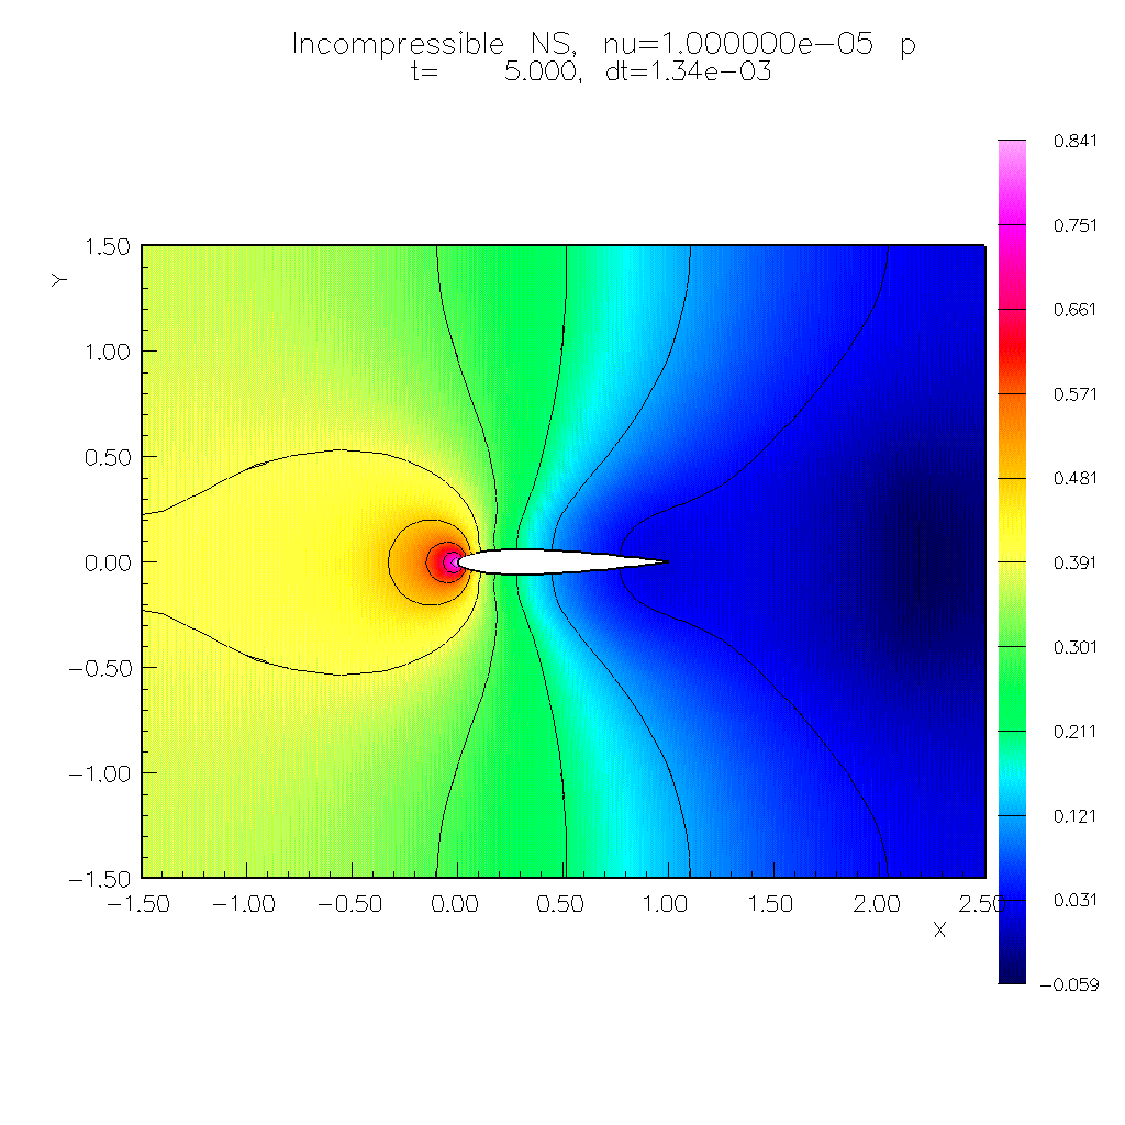
\includegraphics[width=.75\linewidth]{./fig/ins_naca_p}
%- \caption{Incompressible flow past a NACA 0012 airofil.}
%-   \end{center} 
%-   \label{fig:naca}
%- \end{figure}

% The solution is not exactly symmetric but note that the computation of the initial conditions
% through a projection is not currently computed in a symmetric way.

% If you run this example you will notice messages printed to the effect that the \Index{divergence} is
% large on some parts of the grid. By looking at the show file with {\tt plotStuff} and plotting the
% divergence it can be seen that the divergence is large near the leading edge where there are
% large gradients in the solution. This is not unexpected when using artificial diffusion since
% only a minimal amount of smoothing is added. However, it could also indicate
% that either I need a more refined grid there or perhaps a better discretization method such as 
% a finite volume method might work better.

This example demonstrates the use of the second-order non-linear \Index{artificial diffusion} (described in the
Cgins reference guide~\cite{CginsReferenceGuide}). The default value for $\nu=10^{-8}$ is much too
small to have any affect on the solution for the grid being used. 
The value of the artificial diffusion is determined in a local way
that depends on the velocity gradients so as to keep the solution nicely behaved but
with a minimum of dissipation. There is sometimes some fiddling required to get the coefficients
of the artificial diffusion correct. The values are usually always around be $.1$ and $5.$.


% \clearpage
\subsection{Incompressible flow around a moving stirring stick}\index{moving grids!stirring stick}

The command file {\tt cg/ins/cmd/stir.cmd} can be used with cgins to compute the
flow around a rotating tongue depressor.
This example uses the overlapping grid {\tt Overture/\-sampleGrids/\-stir.hdf}  generated
using the command file {\tt Overture/\-sampleGrids/\-stir.cmd}.
\noindent

{
\begin{figure}[hbt]
\newcommand{\figWidtha}{9.cm}
\newcommand{\trimfiga}[2]{\trimPlot{#1}{#2}{.0}{.0}{.08}{.025}}
\begin{center}
\begin{tikzpicture}[scale=1]
  \useasboundingbox (0,.7) rectangle (10,8.2);  % set the bounding box (so we have less surrounding white space)
  \draw ( 0.0,0.0) node[anchor=south west,xshift=-4pt,yshift=+0pt] {\trimfiga{./fig/ob_ins_stir_sl}{\figWidtha}};
% grid:
% \draw[step=1cm,gray] (0,0) grid (10,8.);
\end{tikzpicture}
\end{center} 
 \caption{Incompressible flow around a rotating stirring stick demonstrating the use of moving grids.}
\end{figure}
}

% \begin{figure}[hb]
% \begin{center}
%   % \epsfig{file=\obFigures/ob.ins.stir.sl.ps,width=.75\linewidth} 
%   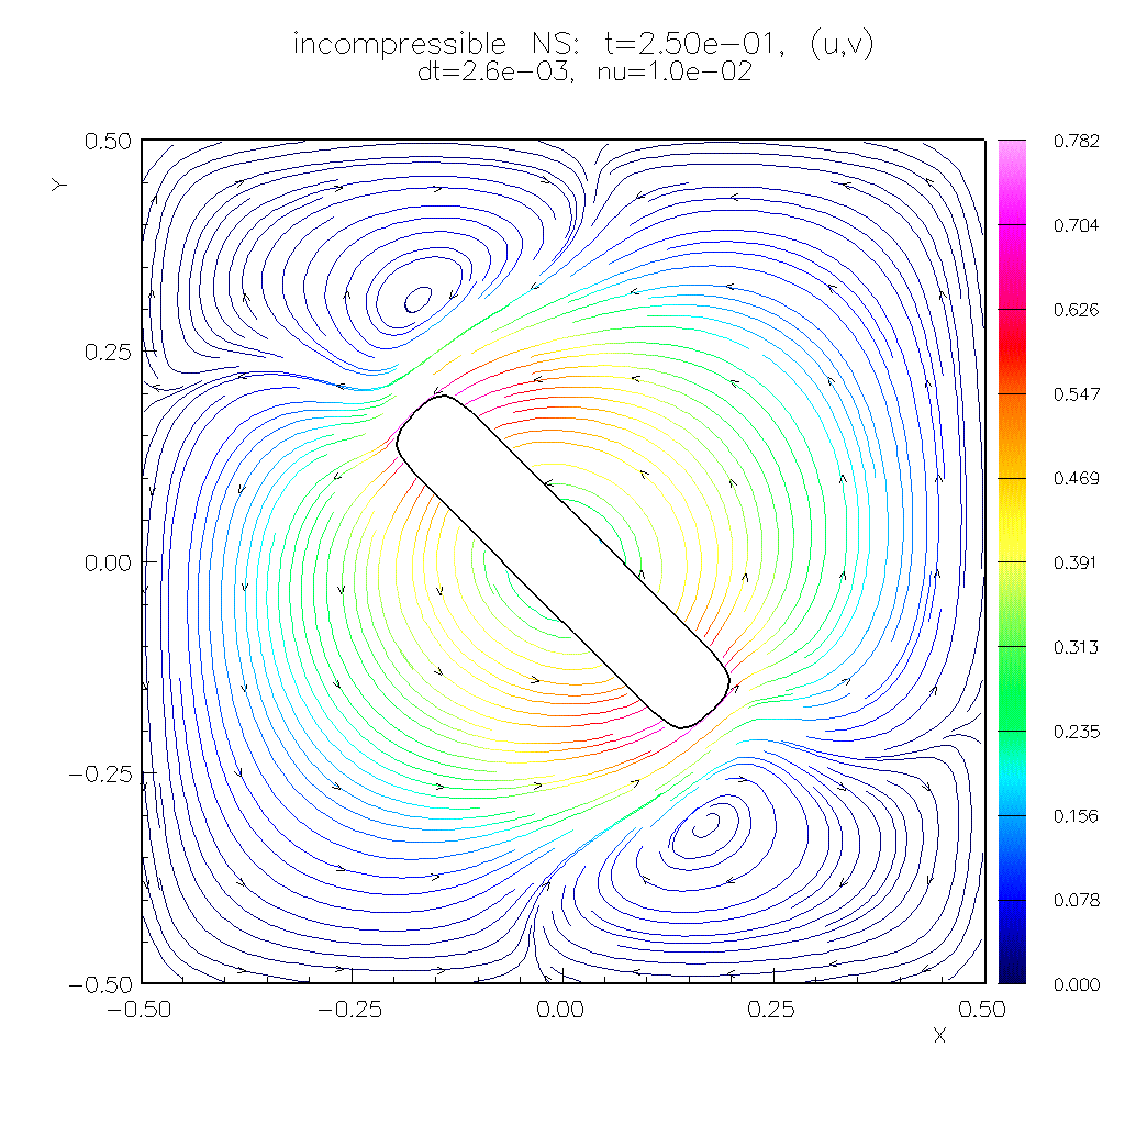
\includegraphics[width=.75\linewidth]{./fig/ob_ins_stir_sl}
%   \end{center}
%   \caption{Incompressible flow around a rotating stirring stick demonstrating the use of moving grids.}
% \end{figure}


% \clearpage
\subsection{Axisymetric incompressible flow past a sphere}\index{axisymmetric}

The command file {\tt cg/ins/cmd/axisym.cmd} can be used to compute the axisymmetric
flow past a sphere. The (two-dimensional) grid can be created with  {\tt Overture/\-sampleGrids/\-halfCylinder.hdf}.
Cgins assumes that the axis of symmetry is the x-axis ($y=0$).


{
\begin{figure}[hbt]
\newcommand{\figWidtha}{12.cm}
\newcommand{\trimfiga}[2]{\trimPlot{#1}{#2}{.15}{.15}{.375}{.375}}
\begin{center}
\begin{tikzpicture}[scale=1]
  \useasboundingbox (0,1) rectangle (12,4.);  % set the bounding box (so we have less surrounding white space)
  \draw ( 0.0,0.0) node[anchor=south west,xshift=-4pt,yshift=+0pt] {\trimfiga{./fig/ins_sphere_axisymmetric_sl}{\figWidtha}};
% grid:
%% \draw[step=1cm,gray] (0,0) grid (12,4.);
\end{tikzpicture}
\end{center} 
 \caption{Incompressible axisymmetric flow past a sphere.}
\end{figure}
}

% \begin{figure}[hb]
% \begin{center}
%   % \epsfig{file=\obFigures/ins.sphere.axisymmetric.sl.ps,width=.75\linewidth} 
%   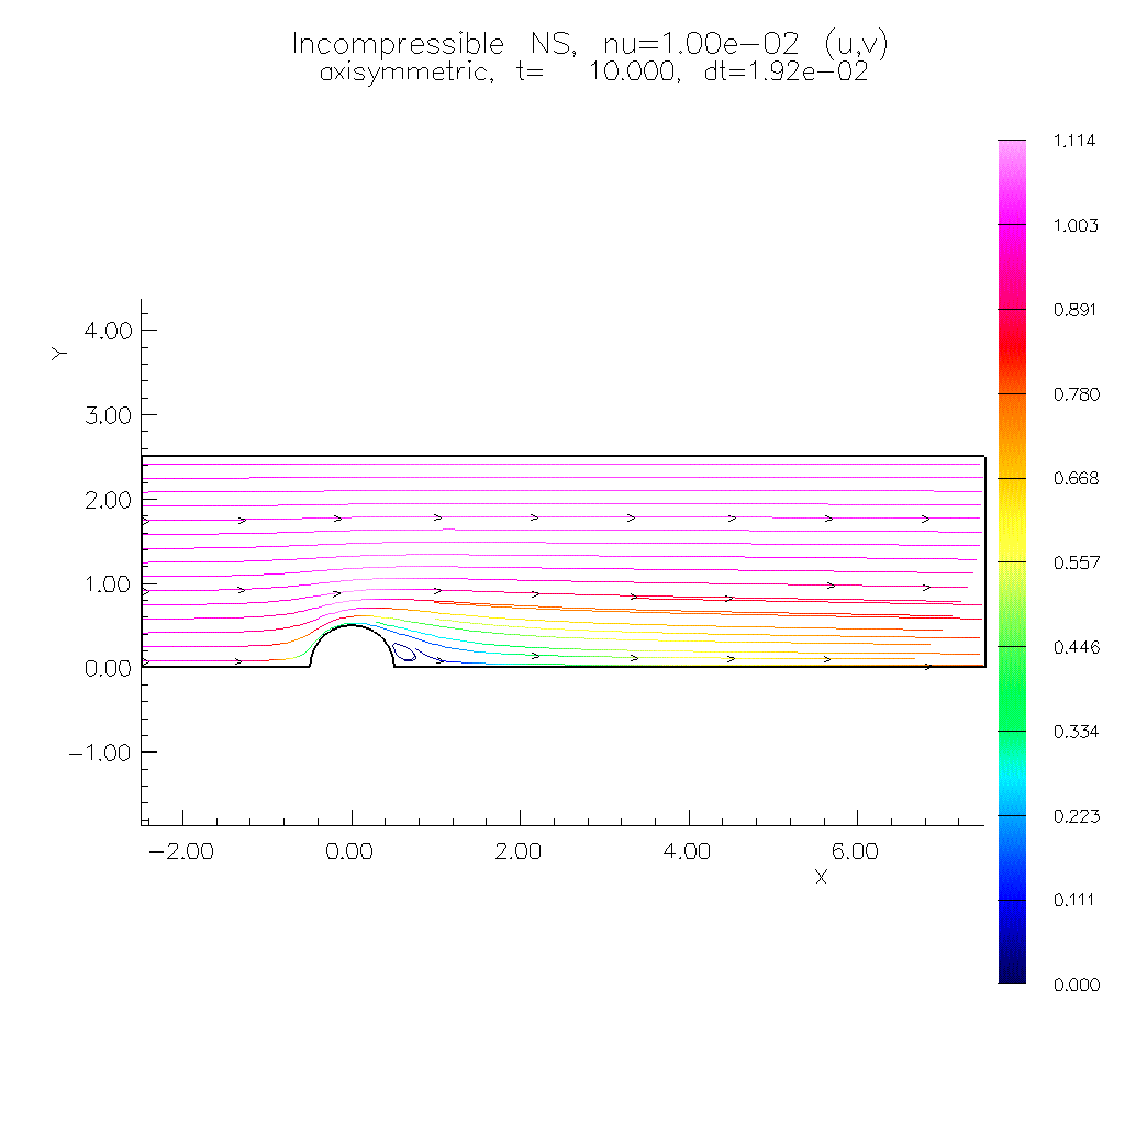
\includegraphics[width=.75\linewidth]{./fig/ins_sphere_axisymmetric_sl}
%   \end{center}
% \vglue-1\baselineskip
%   \caption{Incompressible axisymmetric flow past a sphere.}
% \end{figure}

% \clearpage
\subsection{Incompressible flow past a backward facing step, a C-Grid and an H-grid}
\index{backward facing step}\index{C-grid}\index{H-grid}

The command files {\tt cg/ins/cmd/backStep.cmd}, {\tt cg/ins/cmd/cgrid.cmd} and
{\tt cg/ins/cmd/hgrid.cmd} can be used to solve the problems illustrated in this section.
All of these grids use the {\sl mixed boundary} condition feature, where portions of a 
physical boundary interpolate from another grid. The grids can be generated with the command files
{\tt Overture/sampleGrids/backStep.cmd}, {\tt Overture/sampleGrids/cgrid.cmd} and
{\tt Overture/sampleGrids/hgrid.cmd}.

In general it is preferable NOT to use grids that have been generated with a {\sl mixed boundary}. 
For example, the flow around the convex corner in the backward facing step is not well resolved. 
It is recommended to round off convex corners. See the command file {\tt cg/ins/cmd/backStepSmooth.cmd} 
for flow past a back step with a smoothed corner.

{
\begin{figure}[hbt]
\newcommand{\figWidtha}{8.cm}
\newcommand{\trimfiga}[2]{\trimPlot{#1}{#2}{.02}{.02}{.275}{.4}}
\newcommand{\figWidthb}{8.25cm}
\newcommand{\trimfigb}[2]{\trimPlot{#1}{#2}{.14}{.12}{.35}{.35}}
\newcommand{\figWidthc}{8.cm}
\newcommand{\trimfigc}[2]{\trimPlot{#1}{#2}{.02}{.13}{.05}{.3}}
\newcommand{\figWidthd}{8.cm}
\newcommand{\trimfigd}[2]{\trimPlot{#1}{#2}{.02}{.13}{.125}{.3}}
\begin{center}
\begin{tikzpicture}[scale=1]
  \useasboundingbox (0,.75) rectangle (16.5,8.5);  % set the bounding box (so we have less surrounding white space)
  \draw ( 0.0 ,5.0) node[anchor=south west,xshift=-4pt,yshift=+0pt] {\trimfiga{./fig/backStep}{\figWidtha}};
  \draw ( 8.25,5.5) node[anchor=south west,xshift=-4pt,yshift=+0pt] {\trimfigb{./fig/backStep_sl}{\figWidthb}};
%
  \draw ( 0.0,0.0 ) node[anchor=south west,xshift=-4pt,yshift=+0pt] {\trimfigc{./fig/cgrid_sl}{\figWidthc}};
  \draw ( 8.25,0.0 ) node[anchor=south west,xshift=-4pt,yshift=+0pt] {\trimfigd{./fig/hgrid_vor}{\figWidthd}};
% grid:
%% \draw[step=1cm,gray] (0,0) grid (16.5,8.5);
\end{tikzpicture}
\end{center} 
\caption{Incompressible flow past a backward facing step, a C-grid and an H-grid.}
\end{figure}
}

% \begin{figure}[hb]
% \begin{center}
%   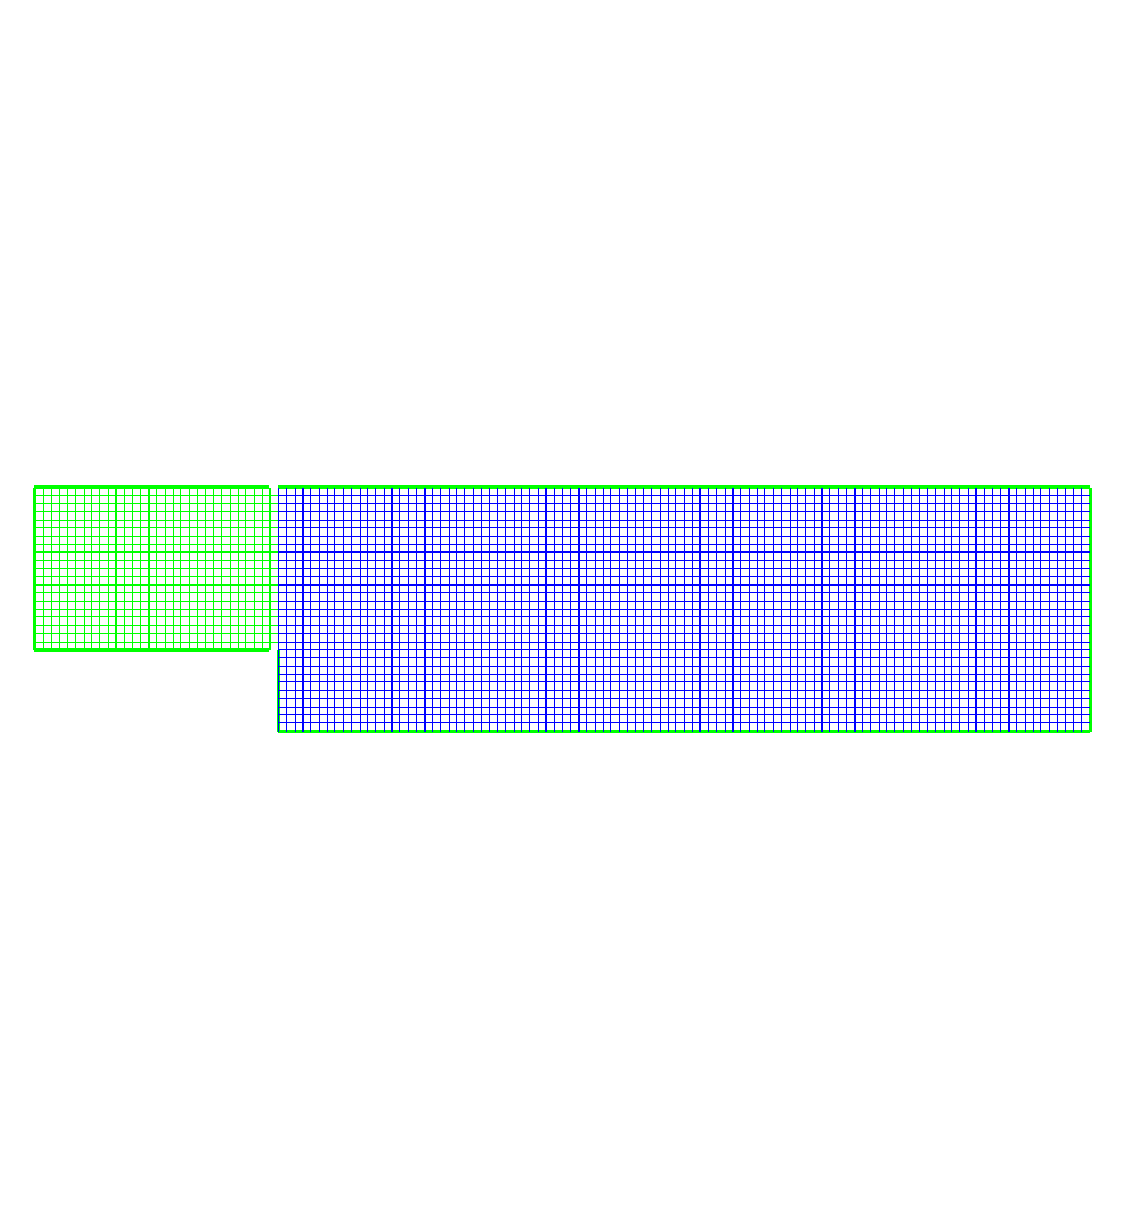
\includegraphics[width=.4\linewidth]{./fig/backStep}
%   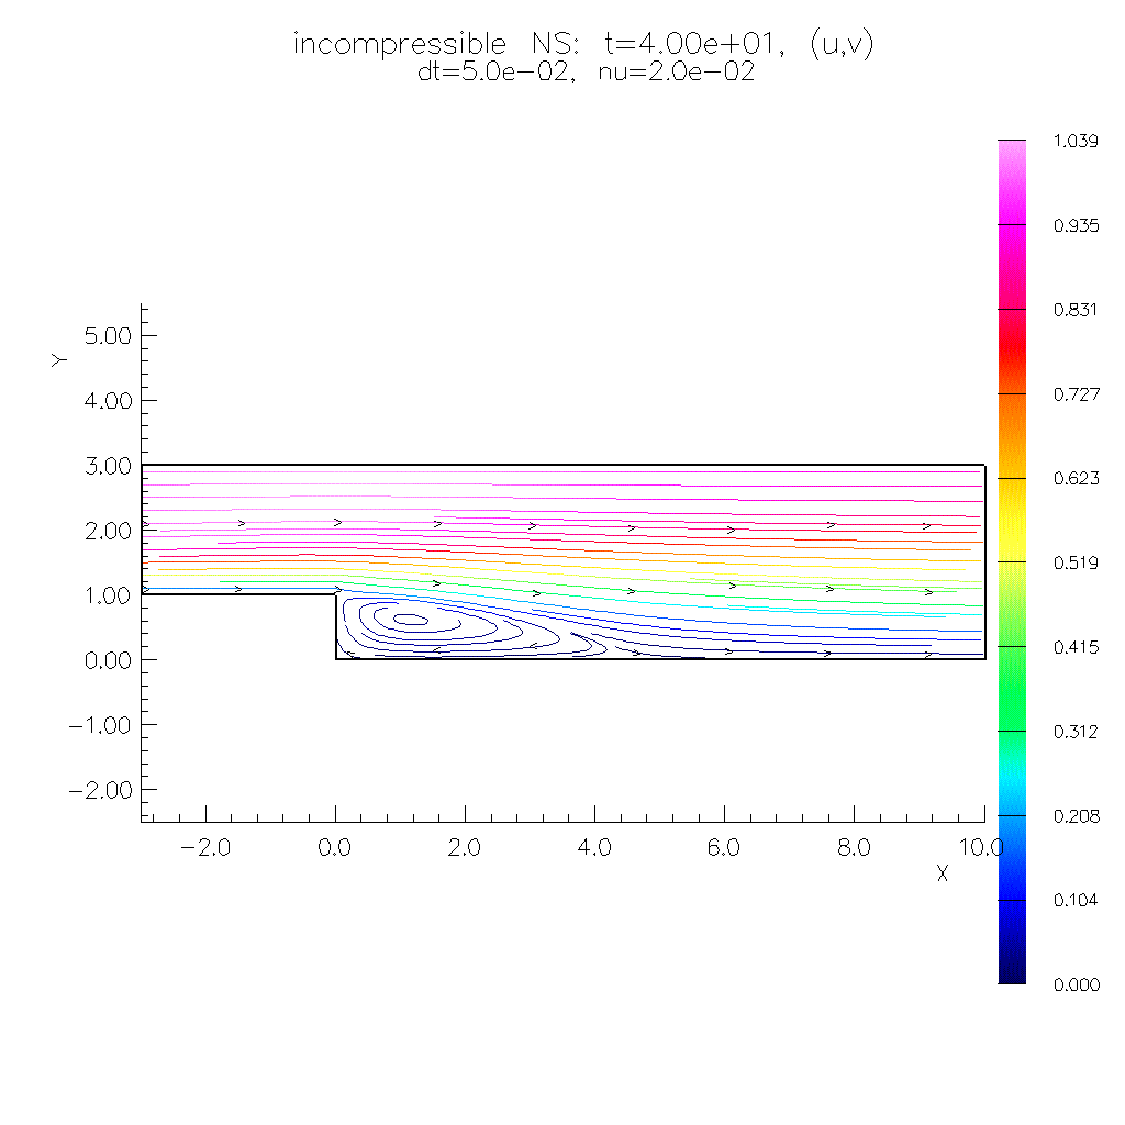
\includegraphics[width=.4\linewidth]{./fig/backStep_sl} \\
%   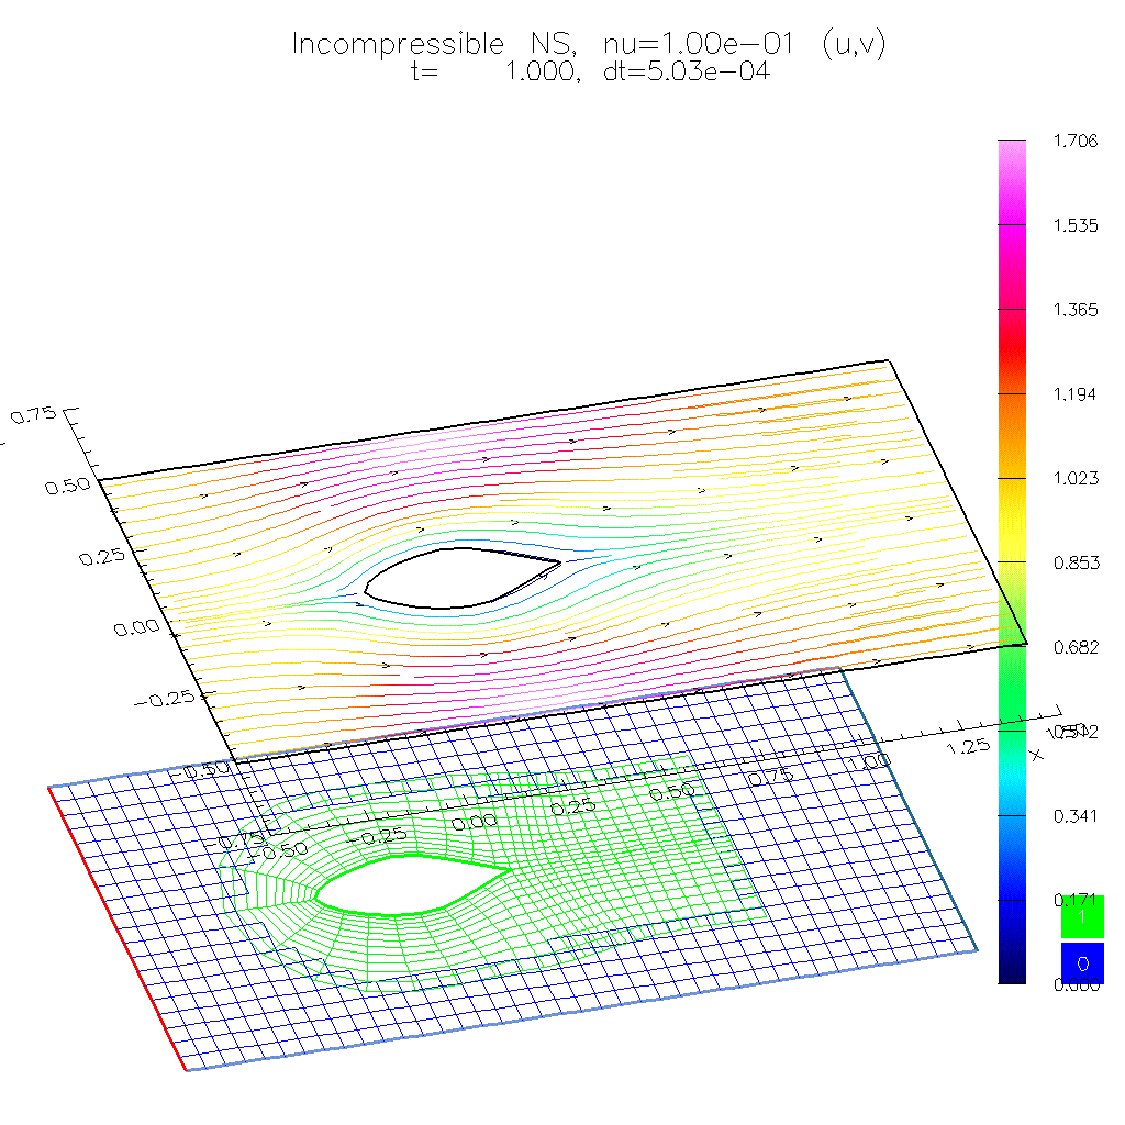
\includegraphics[width=.4\linewidth]{./fig/cgrid_sl}
%   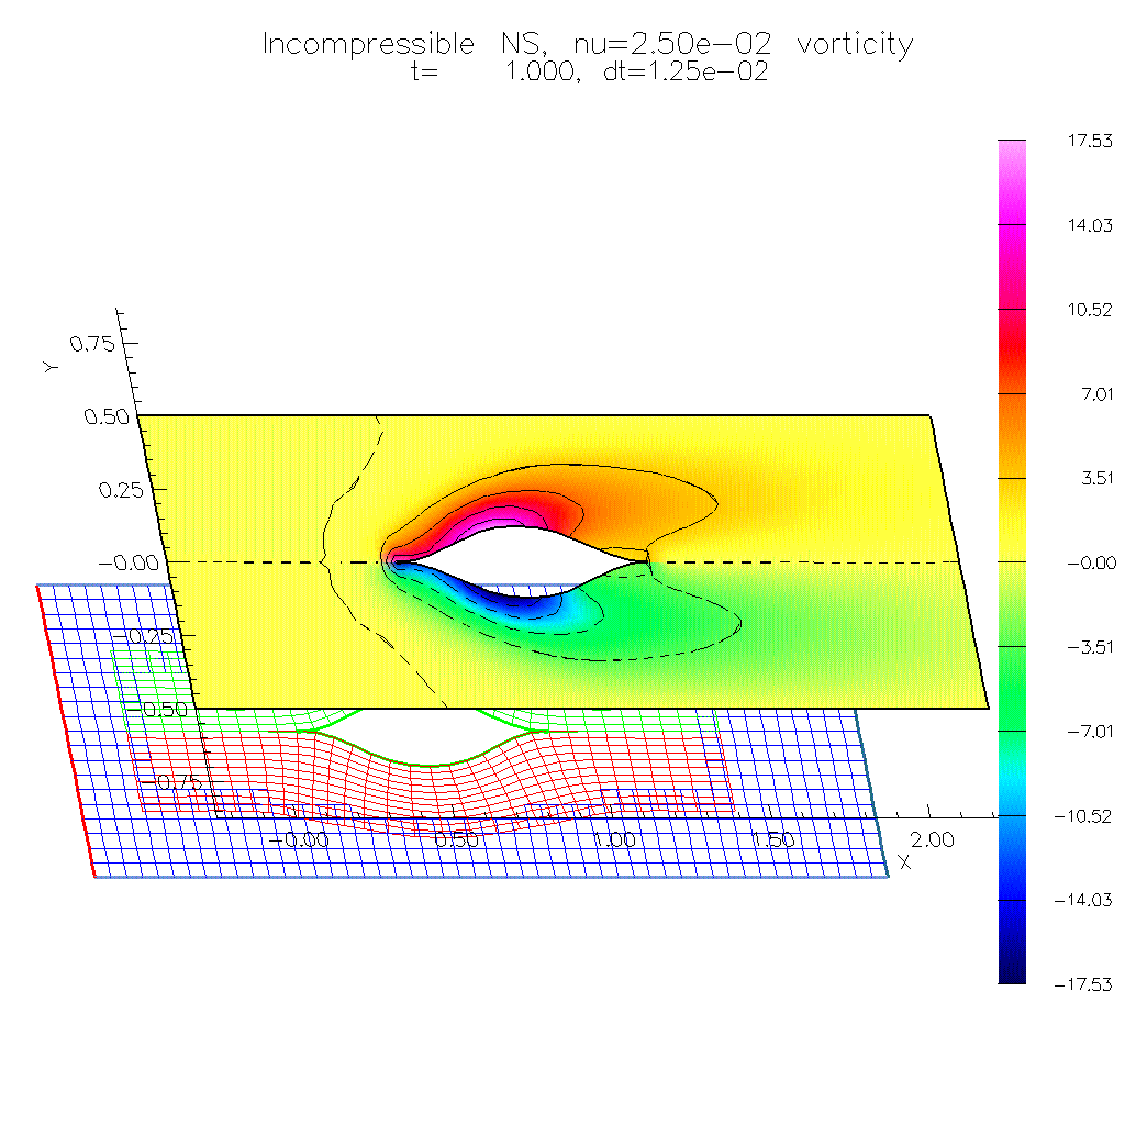
\includegraphics[width=.4\linewidth]{./fig/hgrid_vor}
%   \end{center}
% \vglue-1\baselineskip
%   \caption{Incompressible flow past a backward facing step, a C-grid and an H-grid.}
% \end{figure}



% \clearpage
\subsection{Incompressible flow past a sphere}


The command file {\tt cg/ins/cmd/sib.cmd} can be used with cgins to compute the
flow past a sphere in a box.

{
\begin{figure}[hbt]
\newcommand{\figWidtha}{9.cm}
\newcommand{\trimfiga}[2]{\trimPlot{#1}{#2}{.0}{.0}{.08}{.025}}
\begin{center}
\begin{tikzpicture}[scale=1]
  \useasboundingbox (0,.7) rectangle (9,8.2);  % set the bounding box (so we have less surrounding white space)
  \draw ( 0.0,0.0) node[anchor=south west,xshift=-4pt,yshift=+0pt] {\trimfiga{./fig/ins_sib6_u}{\figWidtha}};
% grid:
%% \draw[step=1cm,gray] (0,0) grid (9,8.);
\end{tikzpicture}
\end{center} 
 \caption{Incompressible flow past a sphere.}
\end{figure}
}

% \begin{figure}[hb]
% \begin{center}
%   % 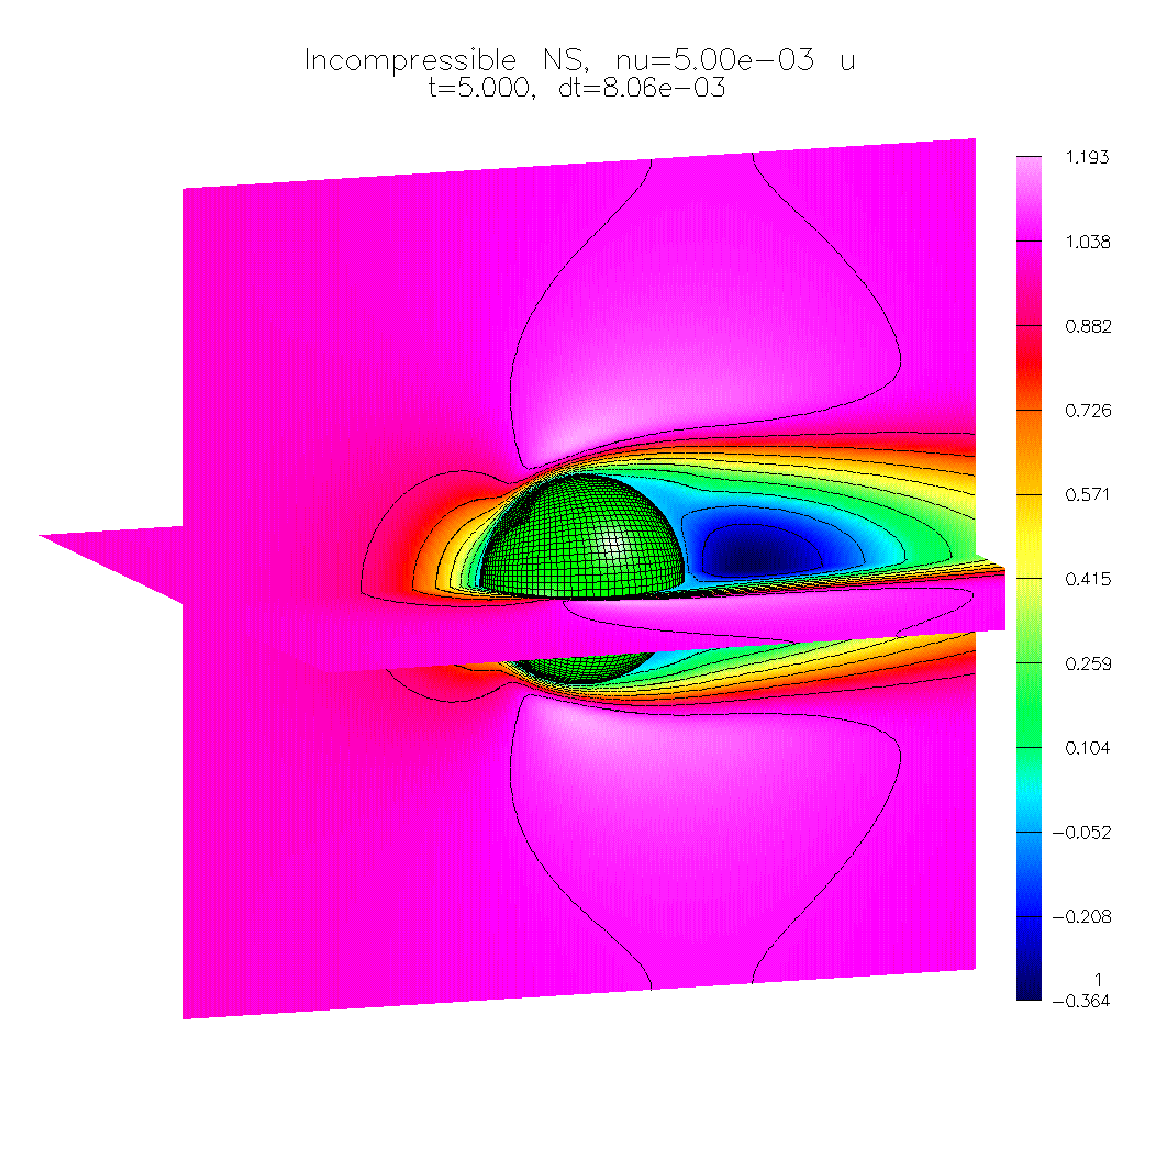
\epsfig{file=fig/ins.sib6.u.ps,width=.75\linewidth} 
%   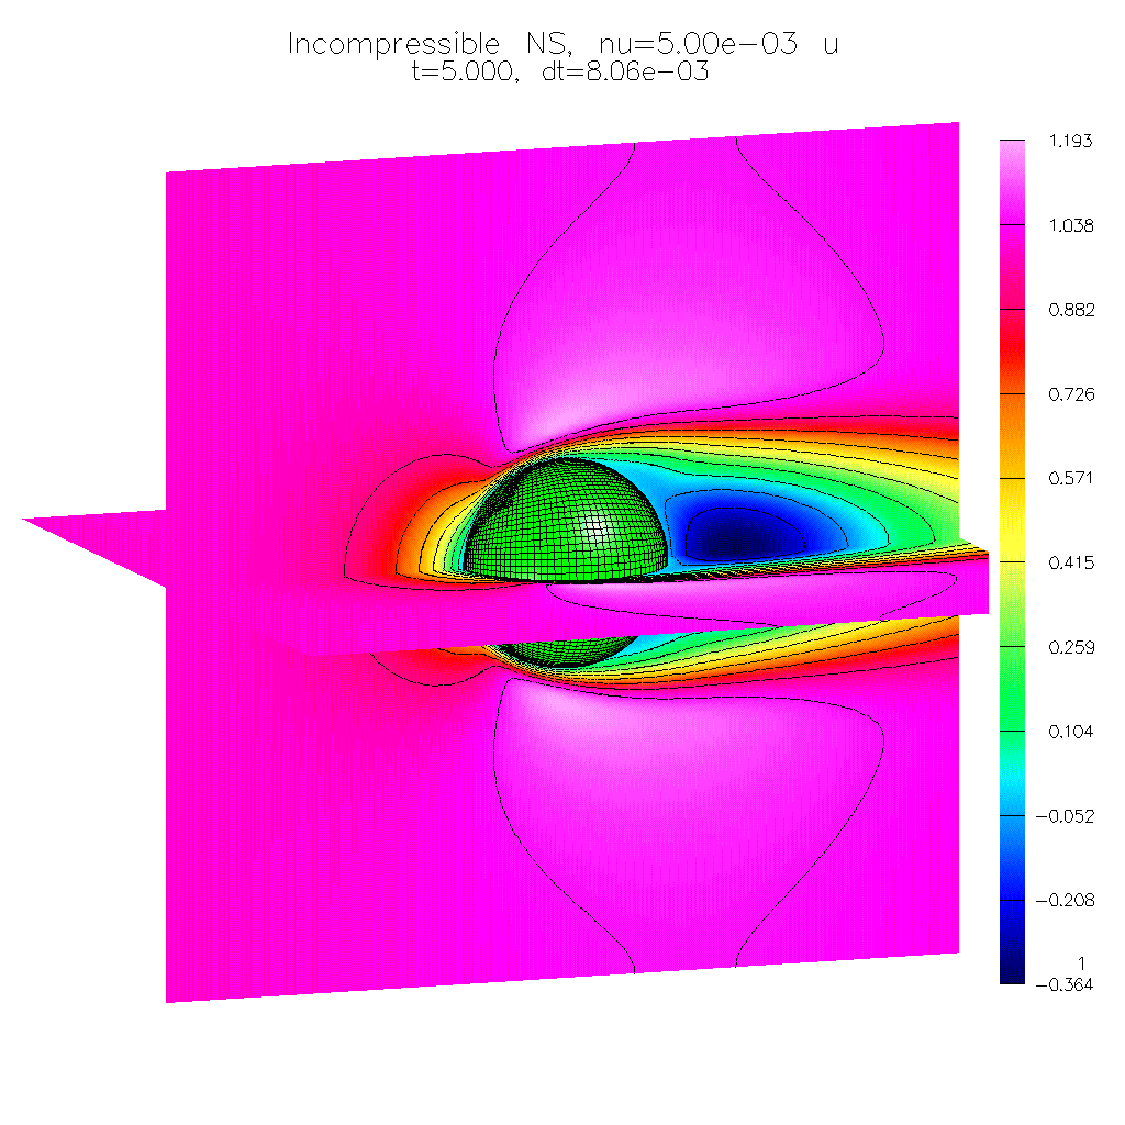
\includegraphics[width=.75\linewidth]{./fig/ins_sib6_u}
%   \end{center}
% \vglue-1\baselineskip
%   \caption{Incompressible flow past a sphere.}
% \end{figure}

% \vspace\baselineskip
For 3D problems it is almost always necessary to use an iterative solver
for the pressure equation and the implicit time stepping equations. The PETSc linear
solvers are recommended. Iterative solvers require a convergence tolerance and you may
have to play around with this tolerance (if the tolerance for the pressure equation
is too large, then the divergence may grow large). 
See the Oges documentation\cite{OGES}
for more information on linear solvers.
% In the above case we use the GMRES solver with a convergence tolerance of
% $10^{-3}$. You may have to play around with this tolerance since I don't
% have a good automatic way to do this yet. 


% \clearpage
\subsection{Incompressible flow through some intersecting pipes}\index{incompressible flow!pipes}

The command file can be {\tt cg/ins/cmd/pipes.cmd} 
used with cgins to compute the flow through two intersecting pipes. The pipes intersect using the
{\em poor man's} intersection option. 
This example uses the overlapping grid {\tt Overture/\-sampleGrids/\-pipes.hdf}  generated
using the command file {\tt Overture/\-sampleGrids/\-pipes.cmd}.
See also the command file {\tt cg/ins/cmd/twoPipes.cmd} where the pipes are joined with a
smooth fillet.

{
\begin{figure}[hbt]
\newcommand{\figWidtha}{9.cm}
\newcommand{\trimfiga}[2]{\trimPlot{#1}{#2}{.0}{.0}{.0}{.025}}
\begin{center}
\begin{tikzpicture}[scale=1]
  \useasboundingbox (0,.7) rectangle (9,9);  % set the bounding box (so we have less surrounding white space)
  \draw ( 0.0,0.0) node[anchor=south west,xshift=-4pt,yshift=+0pt] {\trimfiga{./fig/ins_pipes_p}{\figWidtha}};
% grid:
%\draw[step=1cm,gray] (0,0) grid (9,9.);
\end{tikzpicture}
\end{center} 
\caption{Incompressible flow through some pipes.}
\end{figure}
}


% \begin{figure}[hb]
% \begin{center}
%   % \epsfig{file=\obFigures/ins.pipes.p.ps,width=.75\linewidth} 
%   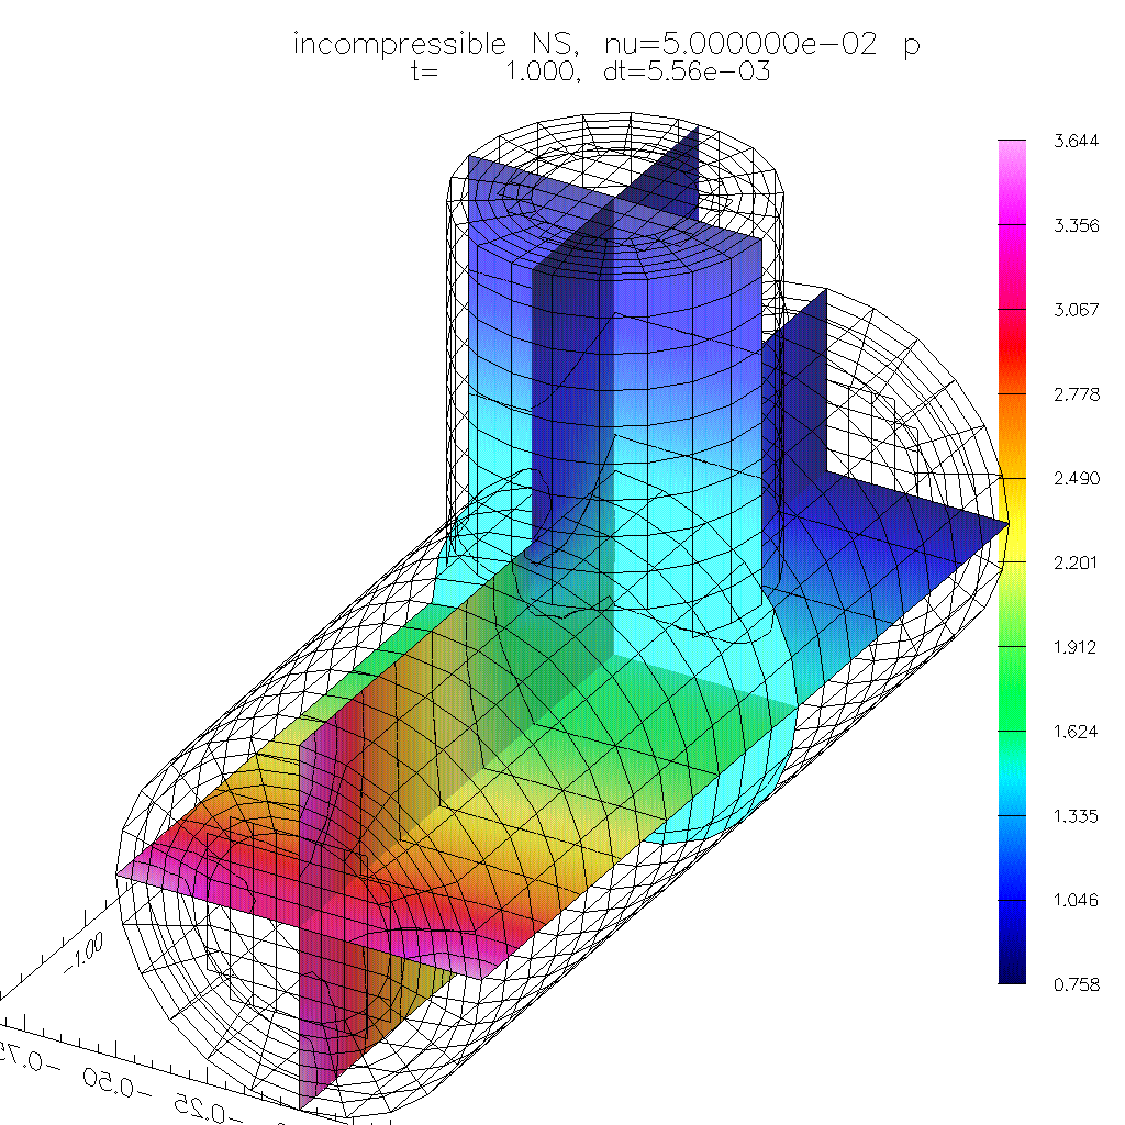
\includegraphics[width=.5\linewidth]{./fig/ins_pipes_p}
%   \end{center}
% \vglue-1\baselineskip
%   \caption{Incompressible flow through some pipes.}
% \end{figure}
% 
\noindent This example demonstrates the use of the parabolic profile for
the inflow boundary condition as described in section~(\ref{sec:parabolic}).


% ---------------------------------
\clearpage
\input twoDrop


\clearpage
% ================================================================================================
\input ../common/specifyingBoundaryConditionsCorrectly.tex



\clearpage
% ===============================================================================================
\section{Options and Parameters} \label{sec:parameters}\index{options}\index{parameters}

There are many options and parameters for \solver. Be warned that not all
combinations of options will work.  It is best to start from an existing command
file and make make minor changes.


% ----------------------------------------------------------------------------------------------------
\subsection{Cgins Setup menu}\label{sec:setupDialog}\index{setup dialog}\index{PDE!choices}

The {\em  Cgins Setup} dialog appears after {\tt cgins} is run and a grid is chosen.
At this point one specifies which PDE to solve.

\noindent The options for {\bf pde} are
\begin{description}
  \item[\qquad incompressible Navier Stokes] : solve the incompressible Navier-Stokes in 2D or 3D or
                 2D-axisymmetric.
\end{description}

\noindent The options for {\bf model} are
\begin{description}
  \item[\qquad standard model] : (default) choose this for the plain vanilla incompressible Navier-Stokes. 
  \item[\qquad Boussinesq model] : temperature dependent flows with buoyancy. 
  \item[\qquad visco-plastic model] : (under development). 
  \item[\qquad two-phase flow model] : (under development). 
\end{description}

\noindent The options for {\bf turbulence model} are
\begin{description}
  \item[\qquad noTurbulenceModel] : (default)
  \item[\qquad Baldwin-Lomax] : under development
  \item[\qquad k-epsilon] : under development
  \item[\qquad k-omega] : under development
  \item[\qquad SpalartAllmaras] : under development
\end{description}

\noindent Other options include:
\begin{description}
  \item[\qquad passive scalar advection] : add an extra passive scalar variable that is advected with the flow.
\end{description}


% --------------------------------------------------------------------------------------------------------------------
\input ../common/parametersDialog.tex

\bogus{
\noindent The {\em } options are
\begin{description}
  \item[\qquad ] : 
\end{description}
}

% -----------------------------------------------------------------------------------------------
\subsubsection{Incompressible NS parameters Dialog (pde options...)}\label{sec:pdeOptions}\index{pde options}

Here is a description of the {\em Incompressible NS parameters Dialog} which defines
options that affect the equations being solved.

\noindent The toggle buttons are
\begin{description}
  \item[\qquad project initial conditions] : project initial conditions to nearly satisfy $\grad\cdot\uv=0$. 
  \item[\qquad second-order artificial diffusion] : turn on/off
  \item[\qquad fourth-order artificial diffusion] : turn on/off
  \item[\qquad sixth-order artificial diffusion] : turn on/off
  \item[\qquad use implicit fourth-order artificial diffusion] : 
  \item[\qquad use split-step implicit artificial diffusion] : 
  \item[\qquad use new fourth order boundary conditions] : 
  \item[\qquad use self-adjoint diffusion operator] : 
  \item[\qquad include artificial diffusion in pressure equation] : 
\end{description}

\noindent The text commands are
\begin{description}
  \item[\qquad nu] : kinematic viscosity (constant).
  \item[\qquad divergence damping] : coefficient of the divergence damping term in the pressure equation.
  \item[\qquad cDt div damping] : scaling coefficient for the divergence damping term when using implicit time
                                   stepping.
  \item[\qquad ad21,ad22] : coefficient of linear and non-linear terms in the second-order artificial diffusion.
  \item[\qquad ad41,ad42] : coefficient of linear and non-linear terms in the fourth-order artificial diffusion.
  \item[\qquad ad61,ad62] : coefficient of linear and non-linear terms in the sixth-order artificial diffusion.
  \item[\qquad kThermal] : thermal diffusivity. 
  \item[\qquad thermal conductivity] : thermal conductivity 
  \item[\qquad passive scalar diffusion coefficient] : coefficient of diffusion for the passive scalar.
\end{description}


% --------------------------------------------------------------------------------------------------------------------
\subsubsection{\Solver\ Time Stepping Parameters Dialog (time stepping parameters...)}
\label{sec:timeSteppingParameters}\index{time stepping parameters}

Here is a description of the {\em \Solver\ Time Stepping Parameters} dialog. These define options
related to time-stepping.

\noindent The options for {\bf method} are the available time-stepping methods. 
The usual choices are one of {\tt adams PC}, {\tt implicit} or {\tt steady state RK-line}. 
\begin{description}
  \item[\qquad forward Euler] :
  \item[\qquad adams order 2] :
  \item[\qquad adams PC] : (default) Adams predictor corrector, order 2.
  \item[\qquad adams PC order 4] :
  \item[\qquad midpoint] :
  \item[\qquad Runge-Kutta] : (does this work?)
  \item[\qquad implicit] : implicit time stepping (other options determine the exact form for this). 
             See {\bf implicitVariation} and {\bf choose grids for implicit}. 
  \item[\qquad variable time step PC] :
  \item[\qquad steady state RK] :
  \item[\qquad steady state RK-line] : pseudo steady-state line solver (very memory efficient). 
\end{description}


\noindent The {\em implicitVariation} options are
\begin{description}
  \item[\qquad implicitViscous] : treat viscous terms only implicitly. 
  \item[\qquad implicitAdvectionAndViscous] : treat viscous and advection terms only implicitly. 
  \item[\qquad implicitFullLinearized] : full implicit method
\end{description}
      

\noindent The {\em accuracy} options are
\begin{description}
  \item[\qquad second order accurate] : second-order accurate in space.
  \item[\qquad fourth order accurate] : fourth-order accurate in space.
\end{description}


\noindent The {\em time accuracy} options specify the accuracy of the time stepping:
\begin{description}
  \item[\qquad solve for steady state] : time accuracy does not matter in this case. 
  \item[\qquad second order accurate in time ] : 
  \item[\qquad fourth order accurate in time ] : 
\end{description}

\noindent The {\em predictor order} options specify the order of the predictor step
for predictor corrector methods: 
\begin{description}
  \item[\qquad default order predictor] :
  \item[\qquad first order predictor] :
  \item[\qquad second order predictor] :
  \item[\qquad third order predictor"] :
  \item[\qquad fourth order predictor"] :
\end{description}

% common parameters are described here: 
\input ../common/commonTimeSteppingParameters.tex


% -----------------------------------------------------------------------------------------------
\input ../common/plotOptions.tex

% -----------------------------------------------------------------------------------------------
\input ../common/outputOptions.tex

% -----------------------------------------------------------------------------------------------
\input ../common/boundaryConditionsOptions.tex

% -----------------------------------------------------------------------------------------------
\input ../common/initialConditionsOptions.tex

% -----------------------------------------------------------------------------------------------
\input ../common/forcingOptions.tex

% -----------------------------------------------------------------------------------------------
\input ../common/twilightZoneOptions.tex

% -----------------------------------------------------------------------------------------------
\input ../common/showfileOptions.tex

% -----------------------------------------------------------------------------------------------
\input ../common/generalOptions.tex

% -----------------------------------------------------------------------------------------------
\input ../common/adaptiveGridOptions.tex

% -----------------------------------------------------------------------------------------------
\input ../common/movingGridOptions.tex

% =================================================================================================
\input ../common/choosingGridsForImplicitTimeStepping.tex

% -------------------------------------------------------------------------------------------------------
\input afsParameters.tex


% --------------------------------------------------------------------------------
\input ../common/runTimeDialog.tex

% -------------------------------------------------------------------------------------------------------
\input ../common/boundaryConditions.tex

% -------------------------------------------------------------------------------------------------------
\input ../common/showFile.tex

% -------------------------------------------------------------------------------------------------------
\input ../common/restart.tex

% -------------------------------------------------------------------------------------------------------
% \input artificialDiffusion.tex 

% =======================================================================================================
\input ../common/userDefinedFunctions.tex


% =======================================================================================================

\section{Hints for running cgins}\index{hints for running}

\begin{itemize}
  \item Start out with a simple problem on a coarse grid so that the problem
      can be quickly run to determine if you have the boundary conditions correct etc.
  \item Start out by taking only a few time steps and looking at the solution to
      see if it looks correct.
  \item The rule of thumb for choosing the viscosity $\nu$ is that if the velocities
    are order 1 and the domain is order 1 then $\nu > h_{\rm max}^2$, where 
    $h_{\rm max}$ is the maximum grid spacing as reported by cgins when it runs.
    This comes from the minimum scale result as discussed in section~(\ref{AD}).
  \item If you want to use as small a viscosity as possible then set $\nu=0$
    and use \Index{artificial diffusion} as discussed in section~(\ref{sec:pdeOptions}).
  \item If cgins blows up it could be the time step is not computed correctly. Reduce
   the cfl parameter (default is .9) to a value like .5 or .25 to see if this is the problem.
   There are known problems with the time step determination for implicit time stepping and
   a large viscosity (relative to the grid spacing).
\end{itemize}

% ===================================================================================================
\section{Trouble Shooting and Frequently asked Questions}\index{trouble shooting}

{\bf Question:} I wonder what is the meaning of this error and what can I do to avoid it.
\begin{verbatim}
computeNumberOfStepsAndAdjustTheTimeStep:ERROR: time step too small? dtNew=1.560026e-61, timeInterval=7.314242e-04
 t=3.699269e+00, tFinal=6.000000e+00, nextTimeToPrint=3.700000e+00, tPrint=1.000000e-03
error
Overture::abort: I am now going to purposely abort so that you can get a traceback from a debugger
Abort
\end{verbatim}

This error usually occurs when the solution develops an instability and gets very
large ({\em blows up} being the technical term). The computed time step will
then be very small. This situation may be caused by a number of factors.

The first thing to do is to look at the solution just before it blows up. If
there are oscillations developing in the interior of the domain or near a
no-slip wall or interpolation boundary then you probably do not have enough
dissipation. Increase the real viscosity $\nu$, or increase the number of grid
points or increase the artificial dissipation and re-run the problem to see if
it runs longer. It could also be that the time step being chosen is too large or
not being re-computed often enough. Decrease the cfl number to see if it has an
effect.  You can also decrease the number of time steps between recomputing the
time step with a command like {\tt recompute dt every 15}. 

The solution may also blow up if the flow enters the domain at an outflow boundary.
This could happen if a strong vortex leaves the domain. You can set the option
{\tt check for inflow at outflow} and then the outflow boundary condition
will be changed if there is inflow detected. You may also be able to 
move the outflow boundary farther downstream to reduce this problem. 


\clearpage
%=================================================================================================
\input ../common/postProcessingAero.tex


% -----------------------------------------------------------------------------------------------------
\subsection{Using PETSc and cgins}\index{PETSc}

  PETSc, the Portable Extensible Toolkit for Scientific computations\cite{petsc-manual},
can be used in cgins to solve implicit systems. 

To use PETSc you should 
\begin{enumerate}
 \item build  PETSc on your machine.
\item define the PETSC\_LIB and PETSC\_ARCH environmental variables (as required to use PETSc normally).
\item edit the file {\tt cg/ins/Makfile} and turn on the PETSc option. 
\end{enumerate}


%=================================================================================================
\vfill\eject
\bibliography{../common/journalISI,../common/henshaw,../common/henshawPapers}
\bibliographystyle{siam}

\printindex

\end{document}


% ----------------------------------------------------------------------------------------------------------



